% !TEX root = dissertation_BB.tex
%% spellcheck-language en-US

%   #
%  ##
%   #
%   #
%  ###

\chapter{Live imaging in three dimensions}

\graphicspath{{./figures/1_spim/}}

Unraveling the secrets of mammalian development has been a long standing challenge for developmental biologists and medical professionals alike. 
% Understanding the early embryonic development allows to shed light on questions such as human infertility and congenital diseases. 
This phase of early life is an incredibly complex and dynamic process spanning through large scales in space and time. Subcellular processes at the nanoscale are happening in the range of milliseconds or faster, while whole embryo reorganizations and tissue migration events take place over the course of hours \cite{gilbert_developmental_2013}. Resolving these processes presents a true challenge, since to understand the underlying mechanisms, molecular specificity is just as crucial as high spatial and temporal resolution.

Light microscopy is one of the oldest methods that is still widely used today to investigate the inner workings of microscopic life. A particularly important branch is fluorescence microscopy \cite{diaspro_optical_2011}, that relies on using fluorescent labels to mark specific regions inside the specimens. Light-sheet microscopy is a relatively new addition to the arsenal of tools that comprise light microscopy methods, and is especially suitable for live imaging of embryonic samples over extended periods of time \cite{keller_quantitative_2008, huisken_selective_2009, weber_light_2011,tomer_shedding_2011}. It is also easily adapted to the sample, allowing to image a large variety of specimens, from entire organs, such as cleared mouse brains \cite{dodt_ultramicroscopy:_2007}, to the subcellular processes occurring inside cultured cells \cite{chen_lattice_2014}.

In an ideal setting, the ultimate microscope would be able to record a continuos, 3D, and multicolor dataset of any biological process of interest with the highest possible resolution. Unfortunately this is not possible; due to several limitations in physics and biology, a compromise is necessary. The diffractive nature of light, the lifetime of fluorescent probes and the photosensitivity of biological specimens all require microscopy to be able to adapt to answer the question at hand. In order to acquire useful data one has to choose a tradeoff between spatial and temporal resolution, and signal contrast, while making sure the biology is not affected by the imaging process itself (Fig. \ref{fig:tradeoffs}) \cite{laissue_assessing_2017}. 

\begin{figure}
  \centering
  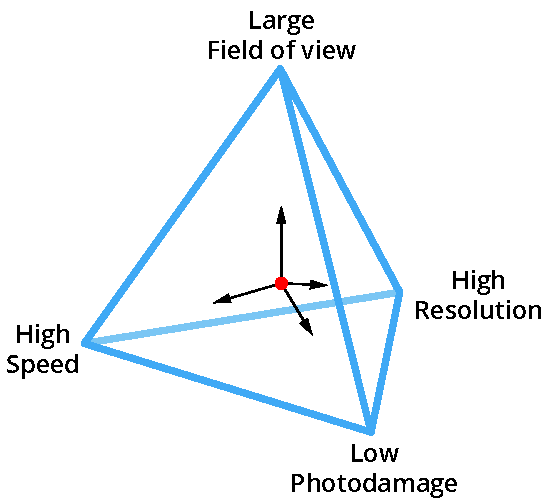
\includegraphics[width=0.6\textwidth]{tradeoffs}
  \bcaption[Tradeoffs in fluorescence microscopy for live imaging]{Also called the ``pyramid of frustration". When optimizing the imaging conditions (red dot), a tradeoff has to be made between resolution, contrast, and imaging speed, while avoiding photodamage. One can only be improved at the expense of the others due to the limited photon budget of the fluorescent molecules. Adapted from \cite{laissue_assessing_2017}.}
  \label{fig:tradeoffs}
\end{figure}

% The most commonly used model organism for these kind of questions is the mouse embryo, that exhibits several common features to human development.
% % , and allows to study it 
% It has several advantages: full genome is sequenced \cite{mouse_genome_sequencing_consortium_initial_2002}, relatively fast reproduction rate facilitating genetic modifications, already extensively developed tools for genetics \cite{capecchi_new_1989,silver_mouse_1995}. All of these make the mouse embryo the primary model organism when investigating biological processes in mammalians.

% Fluorescence microscopy is currently the only imaging technique that not only offers live imaging with high spatial and temporal resolution, it also allows for molecular specificity by the use of fluorescent labeling molecules.



%\section{Light-sheet microscopy}

\section{Wide-field fluorescence microscopy}
  Fluorescence microscopy \cite{lichtman_fluorescence_2005,diaspro_optical_2011}, as a subset of light microscopy is one of the few methods that allows subcellular imaging of live specimens. The first use of the term fluorescence is credited to  George Gabriel Stokes \cite{stokes_change_1852}, and it refers to the phenomenon when a molecule emits light after absorbing light or other electromagnetic radiation. As the name of the technique suggests, this method collects fluorescent light from the specimens which has numerous advantages, but also some drawbacks. Since biological tissue is usually not fluorescent, except for some autofluorescence at shorter wavelengths, fluorescent dyes or proteins have to be introduced to the system in order to be able to collect the necessary information. The advantage of this is that the signal of the labeled structures will be of very high ratio compared to the background.

  A fluorescent molecule is capable of absorbing photons in a given range (excitation spectrum) and temporarily store its energy by having an electron in  a higher energy orbital, \textit{i.e.} in an excited state. This excited state, however is not stable, and the electron quickly jumps back to the ground state while emitting a photon with equal energy to the energy difference between the excited and ground states. The energy of the absorbed and emitted photons are not the same, as energy loss occurs due to internal relaxation events, and the emitted photon has lower energy than the absorbed photon. This phenomenon is called the Stokes shift, or red shift, and can be exploited in microscopy to drastically increase the signal to noise ratio by filtering out the illumination light (Fig. \ref{fig:spectrum}).

  \begin{figure}
    \centering
    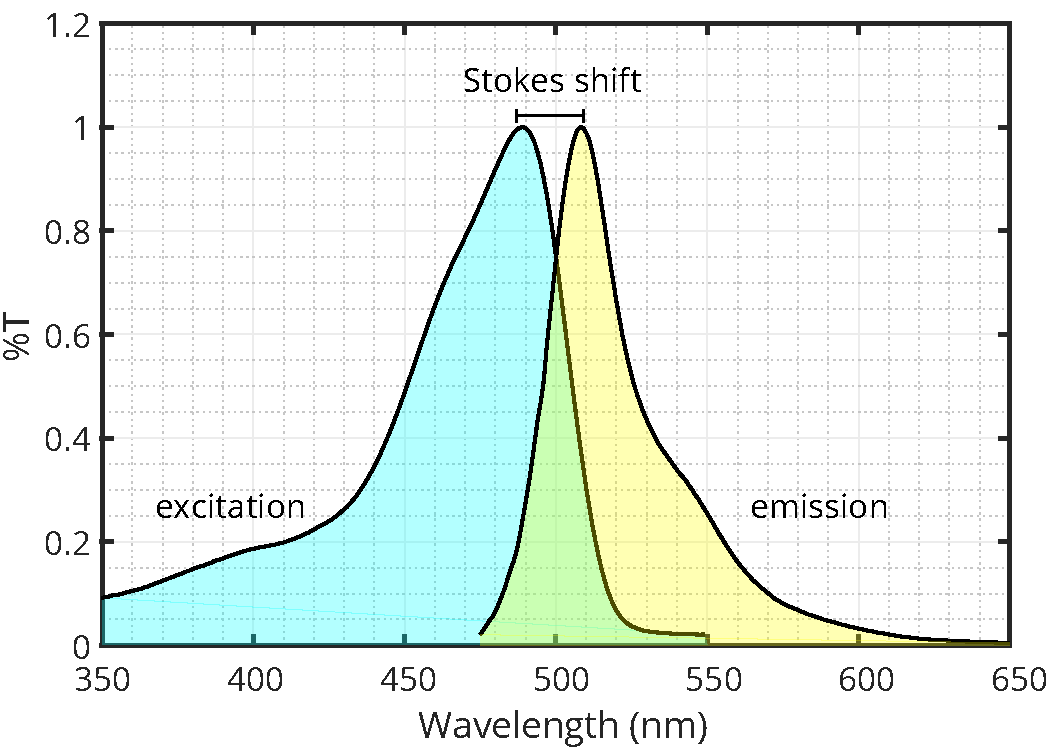
\includegraphics[width=0.6\textwidth]{spectrum/egfp}
    \bcaption[Excitation and emission spectrum of enhanced green fluorescent protein (EGFP)]{Excitation spectrum in blue, emission spectrum in yellow. The separation between the two spectra is due to the Stokes shift, which is 19 nm for EGFP. Emitted and excitation light can be separated by a long-pass filter at \SI{500}{nm}. Data from \cite{noauthor_spectra_nodate}.}
    \label{fig:spectrum}
  \end{figure}

  % Although this process can disturb the natural environment 

  %  very small amount of illumination photons will result in fluorescence ($<0.0001\%$), the signal to noise ratio of the fluorescence is still very high due to the filtering.

  \subsection{Fluorescent proteins}
    Traditionally synthetic fluorescent dyes were used to label certain structures in the specimens. Some of these directly bind to their target,
    % such as DAPI to DNA,
    and others can be used when conjugated to an antibody specific to the structure of interest. The drawback of these methods is that the fluorescent label has to be added to the sample from an external source, and, in many cases, this also necessitates sample preparation techniques incompatible with live imaging, such as fixation \cite{bacallao_guiding_1990}.

    The discovery of fluorescent proteins have revolutionized fluorescence microscopy. Since these molecules are proteins, they can be produced directly by the organism if the proper genetic modifications are performed. Even though this was a hurdle at the time of discovering the green fluorescent protein (GFP) \cite{shimomura_extraction_1962}, the first of its kind, genetic engineering techniques evolved since then \cite{prasher_primary_1992}, and not only has it been successfully integrated in the genome of nematodes \cite{chalfie_green_1994}, zebrafish \cite{amsterdam_aequorea_1995}, and mice \cite{okabe_green_1997}, but many variants have been also engineered by introducing mutations to increase fluorescence intensity, and to change the fluorescence spectrum to allow multicolor imaging \cite{heim_wavelength_1994,heim_engineering_1996,cormack_facs-optimized_1996,okabe_green_1997}. The usefulness and impact of these proteins are so profound, that in 2008 the Nobel Prize in chemistry was awarded to Osamu Shimomura, Martin Chalfie, and Roger Tsien ``for the discovery and development of the green fluorescent protein, GFP" \cite{service_three_2008}.


  \subsection{Wide-field image formation}
    By imaging fluorescently labelled specimens, a wide-field fluorescence microscope has the capability of discriminating illumination light from fluorescent emitted light due to the Stokes shift described in the previous section. The microscope's operating principle is depicted in Figure \ref{fig:wide-field}.

    A light source, typically a mercury lamp is focused on the back focal plane of the objective to create even illumination at the sample. Before entering the objective, the light is filtered, so only the wavelengths that correspond to the excitation properties of the observed fluorophores are transmitted. Since the same objective is used for both illumination and detection, a dichroic mirror is utilized to decouple the illumination and detection paths. The emitted light is filtered again to make sure any reflected and scattered light from the illumination source is blocked to increase signal to noise ratio.

    Finally, the light is focused by a tube lens to create a magnified image in the camera sensor. This type of imaging is called infinity corrected optics, since the back focal point of the objective is in ``infinity", meaning that the light exiting the back aperture is parallel. This is achieved by placing the sample exactly at the focal point of the objective. Infinity corrected optics has the advantage that it allows placing various additional optical elements in the infinity space (\textit{i.e.} the space between the objective and the tube lens) without affecting the image quality. In this example such elements are the dichroic mirror and the emission filter. 

    \begin{figure}[tb]
      \centering
      \includegraphics[page=4,width=0.7\textwidth]{spim_cyl}
      \bcaption[Wide-field fluorescence microscope]{(a) The light source is focused on the back focal plane of the objective to provide an even illumination to the sample. Emitted photons are collected by the objective, and are separated from the illumination light by a dichroic mirror. (b) , $\alpha$}
      \label{fig:wide-field}
    \end{figure}


    The combination of the objective and tube lens together will determine the magnification of the system, it will be the ratio of the focal lengths of these lenses:
    \begin{equation}
      M = \frac{f_{TL}}{f_{OBJ}}.
      \label{eq:magnification}
    \end{equation}
    The final field of view (FOV) of the microscope will depend on the magnification, and also on the size of the imaging sensor:
    \begin{equation}
      FOV = \frac{A}{M},
      \label{eq:FOV}
    \end{equation}
    where $A$ is the area of the sensor. 

    Apart from magnification, the most important property of the objective is the half-angle of the light acceptance cone, $\alpha$. This not only determines the amount of collected light, but also the achievable resolution of the system (see next section). This angle depends on the size of the lens relative to its focal length. In other words depends on the aperture of the lens, which is why the expression \textit{numerical aperture} (NA) is more commonly used to express this property of the objective:
    \begin{equation}
      \text{NA} = n\cdot \sin \alpha.
      \label{eq:NA}
    \end{equation}

    For small $\alpha$ angles, the following approximation holds true: $\sin \alpha \approx \tan \alpha \approx \alpha$. Thus, the numerical aperture can also be expressed as a ratio of the radius of the lens and the focal length:
    \begin{equation}
      NA \approx n \frac{r}{f},\quad \text{when }\alpha \ll 1.
    \end{equation}
    % This expression also shows the relationship of the numerical aperture and the f-number commonly used in photography to characterize a lens' aperture:
    % \begin{equation}
    %     f\# = \frac{f}{d} \approx \frac{2}{n\cdot NA}
    % \end{equation}


    % ########  ########  ######  
    % ##     ## ##       ##    ## 
    % ##     ## ##       ##       
    % ########  ######    ######  
    % ##   ##   ##             ## 
    % ##    ##  ##       ##    ## 
    % ##     ## ########  ######  

  \subsection{Resolution of a wide-field microscope}
    The resolution of an optical systems is defined by the size of the smallest distinguishable feature on the image. Practically this means the minimum distance between two point-like objects so that the two objects can still be resolved. This mainly depends on two factors: the NA of the objective, and the pixel size of the imaging sensor.

    Even if the imaging sensor would have infinitely fine resolution, it is not possible to reach arbitrary high resolutions due to the wave nature of light and diffraction effects that occur at the aperture of the objective. This means that depending on the wavelength of the light, any point source will have a finite size on the image, it will be spread out, that will limit the resolution. The shape of this image is called the \textit{point spread function}, or PSF (Fig. \ref{fig:psf-wf}), as this function describes the behavior of the optical system when imaging a point like source. This property of lenses was already discovered by Abbe in 1873 \cite{abbe_beitrage_1873}, when he constructed his famous formula for resolution:
    \begin{equation}
      \delta = \frac{\lambda}{2 \cdot NA}.
      \label{eq:abbe}
    \end{equation}
    where $d$ is the smallest distance between two distinguishable features.

    Another representation of the optical performance, is the \textit{optical transfer function}, or OTF (Fig. \ref{fig:psf-wf}), which is the Fourier transform of the PSF:
    \begin{equation}
      \text{OTF} = \mathcal{F}(\text{PSF}).
    \end{equation}
    As this function operates in the frequency space, it describes how the different frequencies are affected by the system. The resolution can also be defined as the support of the OTF, since this describes the highest frequency that is still transmitted through the optical system. Any pattern with higher frequency will be lost, thus beyond the resolution limit. For circularly symmetric PSFs, the OTF will be real valued, however if this is not the case, the Fourier transform also introduces complex components.

    \begin{figure}
      \centering
      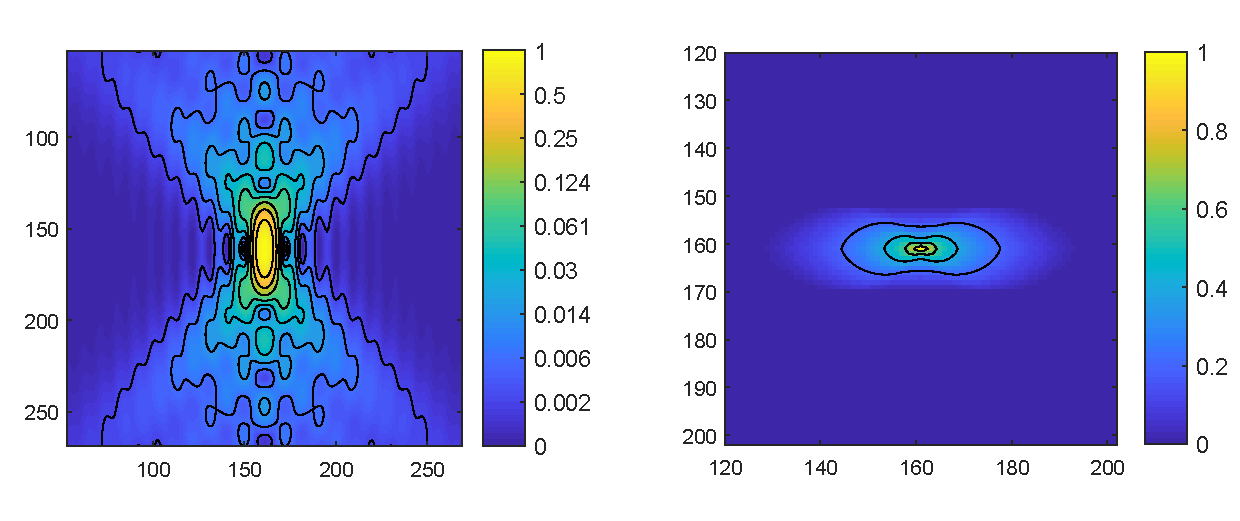
\includegraphics[width=1\textwidth]{psfs/WF.pdf}
      \bcaption[Axial cross section of the PSF and OTF of a wide-field microscope]{Simulated PSF and OTF for a wide-field microscope with a water immersion objective ($n=1.33$). $NA=1.1$, $\lambda = \SI{510}{nm}$}
      \label{fig:psf-wf}
    \end{figure}


    Abbe's formula can be derived from the scalar theory of diffraction using a paraxial approximation (Fraunhofer diffraction, \cite{born_principles_2013}) that describes the intensity of the electric field in the focus of a lens \cite{sheppard_imaging_1987}:

    \begin{equation}
      H(u,v) = C_0 \left| \int_0^1 J_0 (vr)e^{-i\frac{1}{2}\cdot ur^2} rdr \right|^2,
      \label{eq:psf}
    \end{equation}
    where $C_0$ is a normalization constant, and $J_0$ is the zero order Bessel function of the first kind. Furthermore, instead of the commonly used Cartesian coordinates $x$, $y$ and $z$, the following optical coordinates are defined:
    \begin{equation}
      v = \frac{2\pi n  r}{\lambda_0} \sin \alpha, \quad
      u=\frac{8\pi n  z}{\lambda_0} \sin^2 \frac{\alpha}{2}
      \label{eq:substitutions}
    \end{equation}
    where $r = \sqrt{x^2 + y^2}$ is the distance from the optical axis, and $\alpha$ is the light collection angle as shown on Fig. \ref{fig:wide-field}. 

    To determine the lateral resolution of the system, let's substitute $u=0$ as the axial optical coordinate, and evaluate Eq. \ref{eq:psf} which will give the intensity distribution in the focal plane:
    \begin{equation}
      H(0,v) = C_0 \left| \int_0^1 J_0(vr)rdr \right|^2 = \left(2\frac{J_1(v)}{v} \right) ^2,
      \label{eq:airy}
    \end{equation}
    \begin{figure}
      \centering
      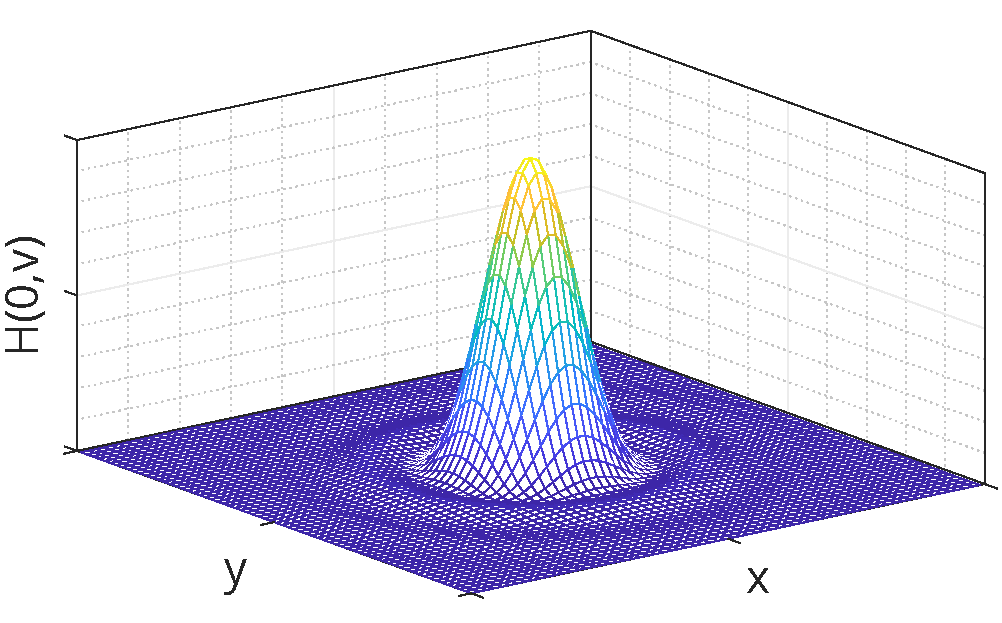
\includegraphics[width=0.7\textwidth]{airy}
      \bcaption[Airy pattern]{Airy pattern calculated in Matlab based on Eq. \ref{eq:airy}}
      \label{fig:airy}
    \end{figure}


    

    where $J_1$ is the first order Bessel function of the first kind. This equation describes the famous Airy pattern (Fig. \ref{fig:airy}) which will be the shape of the PSF in the focal plane. The width of this pattern is the resolution, and although there are multiple definitions for this, the most commonly accepted is the Rayleigh criterion \cite{f.r.s_xxxi._1879, born_principles_2013} which defines the resolution as the distance between the central peak and the first local minimum. As this lies at $v=3.38$, the resolution can be expressed by substituting this value to Eq. \ref{eq:substitutions} and calculating the real distance ($r$):
    \begin{equation}
      \delta_{xy} = \frac{3.83}{2\pi} \frac{\lambda_0}{n\cdot \sin \alpha} \approx 0.61 \frac{\lambda_0}{NA},
      \label{eq:lateralRes}
    \end{equation}
    which is equivalent to Abbe's original formula (Eq. \ref{eq:abbe}). The only difference is the scaling factor which is due to the slightly different interpretations of width of the Airy disk as mentioned earlier.

    Similarly, to calculate the intensity distribution along the axial direction, let's substitute $v=0$ to Eq. \ref{eq:psf}:
    \begin{equation}
      H(u,0)=C_0\left( \frac{\sin \frac{u}{4}}{\frac{u}{4}}\right) ^2 . 
    \end{equation} 
    For this expression the first minimum lies at $u=4\pi$. Converting back to Cartesian coordinates, the axial resolution can be expressed as:
    \begin{equation}
      \delta_z = \frac{2n\lambda_0}{NA^2}.
      \label{eq:axialRes}
    \end{equation}

    So far we only considered a single, point-like emitter. As the intensity function describes how an optical system ``spreads out" the image of a point, it is also called the Point Spread Function (PSF, Fig. \ref{fig:psf-wf}). In a more realistic scenario, however the emitters are neither point-like, nor single. Effectively, however, for every emitter the PSF would be imaged on the sensor, and this creates the final image. In mathematical terms, this can be expressed as a convolution operation between the underlying fluorophore distribution of the object ($O$) and the PSF ($H$):
    \begin{equation}
      I(u,v) = O(u,v) * H(u,v).
    \end{equation}

    The effective result of this kind of diffraction limited image formation is a blurred image with a finite resolution of $\delta_{xy}$ in the lateral direction, and $\delta_z$ in the axial direction.

    The PSF is further affected by the illumination pattern as well. Since the number of emitted fluorescent photons are roughly proportional to the illumination intensity, if the illumination has any structure at the order of the detection resolution, it will have an effect on the overall PSF of the system, which can be expressed as:
    \begin{equation}
      H_{sys} = H_{ill} \cdot H_{det},
      \label{eq:systemPSF}
    \end{equation}
    where $H_{ill}$ is the point spread function of the illumination, and $H_{det}$ is the point spread function of the detection.



\section{Point scanning methods}
  In most cases, a wide-filed microscope is used to image a section of a tissue, thus axial resolution is not a concern. Imaging live specimens, however is not so straightforward, as these samples are usually much thicker than a typical section. For these samples 3-dimensional (3D) imaging is highly beneficial, which necessitates some kind of optical sectioning technique to be able to discriminate the features at different depths.


  Due to the design of the wide-field microscope, any photons emitted from outside the focal plane will also be detected by the sensor, however as these are not originating from the focus, only a blur will be visible. This blur potentially degrades image quality and signal-to-noise ratio to such extent that makes imaging thick sample very difficult if not impossible in a wide-field microscope. 

  % In the previous section we defined optical resolution, and derived the formulas to calculate the lateral and axial resolutions. These formulas, however are not completely accurate for high NA imaging, since the derivation itself depended on a paraxial approximation of the Kirchhoff diffraction equation. A more robust, and generally accepted method to calculate the resolution for high-NA objectives is the Stelzer-Grill-Heisenberg (SGH) theory
  % \cite{grill_method_1999, stelzer_uncertainty_2000}:
  % \begin{equation} \label{eq:latres}
  % \sigma_{xy}=\frac{\lambda}{\sqrt{3-2 \cos \alpha - \cos 2 \alpha}}
  % \end{equation}
  % \begin{equation} \label{eq:axres}
  % \sigma_z = \frac{\lambda}{1-\cos \alpha}
  % \end{equation}

  \begin{figure}
    \centering
    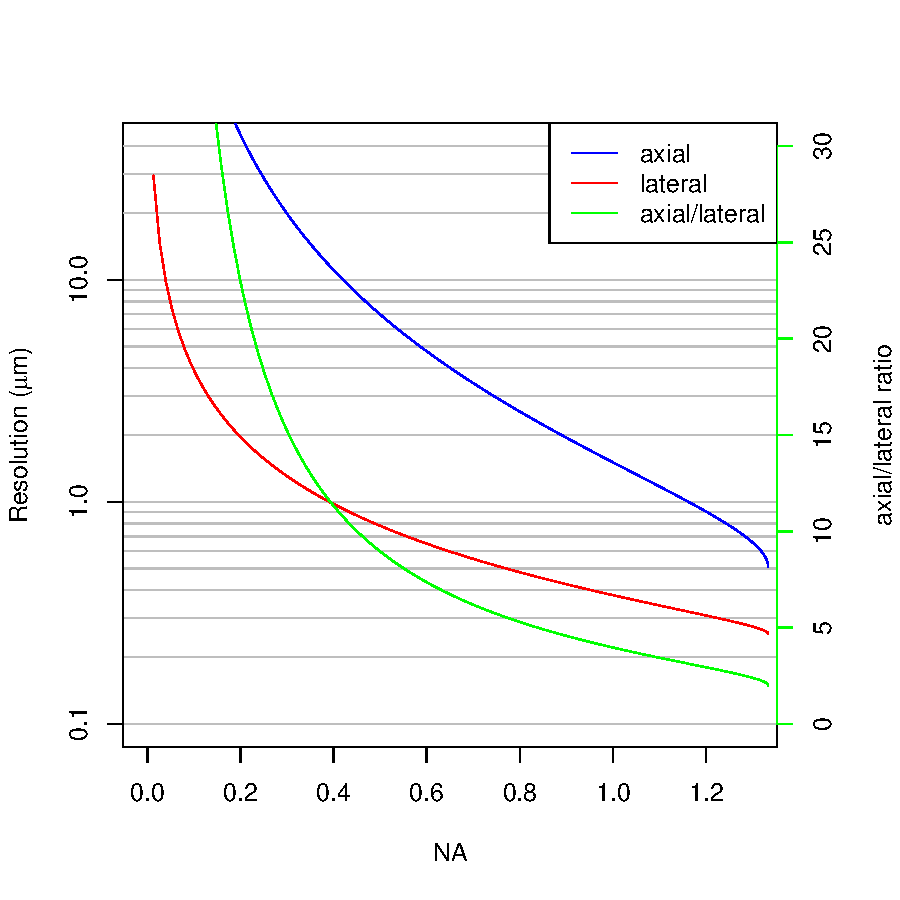
\includegraphics[width=0.6\textwidth]{resolution}
    \bcaption[Resolution of a wide-field microscope]{Axial (blue) and lateral (red) resolutions of a wide-field microscope are shown with respect to the numerical aperture (NA). Resolutions are calculated with $\lambda =510nm$, the emission maximum of GFP and $n=1.33$, the refractive index of water, for water dipping objectives.}
    \label{fig:resolution}
  \end{figure}

  Evaluating Equations \ref{eq:lateralRes} and \ref{eq:axialRes} for a range of possible numerical apertures reveals the significant differences in lateral and axial resolution for any objective (Fig.~\ref{fig:resolution}). Especially for low NAs, this can be significant, a factor of $\sim$20 difference. For higher (>0.8) NAs the axial resolution increases faster than the lateral, however they will only be equal when $\alpha=\SI{180}{\degree}$. This means that isotropic resolution with a single lens is only possible if the lens is collecting all light emitting from the sample, which seems hardly possible, and would be highly impractical. For commonly used high NA objectives the lateral to axial ratio will still be around 3--6. 

  Instead of using a single lens to achieve isotropic resolution, it is more practical to image the sample from multiple directions to complement the missing information from different views. When rotating the sample \SI{90}{\degree} for example, the lateral direction of the second view will correspond to the axial direction of the first view. If rotation is not possible, using multiple objectives can also achieve similar result, such as in the case of Multi-Imaging Axis Microscopy (MIAM) \cite{swoger_multiple_2003,swoger_multi-view_2007}. This microscope consisted of 4 identical objectives arranged in a tetrahedral fashion to collect as much light as possible from multiple directions, and provide isotropic 3D resolution, albeit at the expense of extremely difficult sample handling, since the sample was completely surrounded by objectives from all directions. 

  % Another disadvantage of the wide-field microscope, is that it can not be used with thick specimens. Usually this type of microscopy is only used for a single layer of cells, because all the objects in the field of view will appear on the imaging plane, not just the plane in focus. These objects will appear blurred if close to the focus, or just evenly add to the background noise if they are further from the focus. This is why imaging specimens much thicker than $10\ \mu m$ will result in suboptimal image quality.





%  ####    ####   #    #  ######   ####    ####     ##    #      
% #    #  #    #  ##   #  #       #    #  #    #   #  #   #      
% #       #    #  # #  #  #####   #    #  #       #    #  #      
% #       #    #  #  # #  #       #    #  #       ######  #      
% #    #  #    #  #   ##  #       #    #  #    #  #    #  #      
%  ####    ####   #    #  #        ####    ####   #    #  ###### 
                                                              

  \subsection{Confocal laser scanning microscopy}

    Confocal laser scanning microscopy (CLSM) \cite{minsky_microscopy_1961,davidovits_scanning_1969} addresses most of the problems of wide-field microscopy we mentioned in the previous section. It is capable of optical sectioning by rejecting out of focus light, which makes it a
    true % what?
    3D imaging technique. Furthermore, the light rejection also massively reduces out of focus background, and increases contrast.

    This is achieved by two significant modifications compared to the wide-field optical path. To be able to reject the out of focus light, an adjustable pinhole is placed at the focus of the tube lens. Light rays originating from the focal point will meet at this position, and are able to pass through the pinhole, however out-of-focus light will converge either before or after the aperture, and thus the aperture blocks these rays. To maximize the fluorescence readout efficiency for the single focal point, a photomultiplier tube is used instead of an area sensor (Fig. \ref{fig:confocal}).

    \begin{figure}[tb]
    \begin{subfigure}[t]{0.49\textwidth}
      \centering
      \includegraphics[page=3,width=\textwidth]{spim_cyl}
      \caption{\textbf{Confocal microscope}}
      \label{fig:confocal}
    \end{subfigure}
    \begin{subfigure}[t]{0.49\textwidth}
      \centering
      \includegraphics[page=5,width=\textwidth]{spim_cyl}
      \caption{\textbf{Confocal-theta microscope}}
      \label{fig:conf-theta}
    \end{subfigure}
    \bcaption[Basic optical components of a confocal laser scanning and confocal-theta microscope]{Both type of microscopes use confocal images detection, which means that a pinhole is used to exclude light coming from out of focus points. Light intensity is measured by a photomultiplier for every voxel in the region of interest. The final image is generated on a computer using the positions and recorded intensity values. A regular confocal microscope (\ref{fig:confocal}) uses the same objective for illumination and detection, while a confocal-theta microscope (\ref{fig:conf-theta}) uses a second objective that is rotated by $\vartheta$ around the focus. In this case, $\vartheta = 90^\circ$.}
    \label{fig:confocals}
    \end{figure}

    To maximize the signal from the focal point, the illumination light is also focused here by coupling an expanded laser beam through the back aperture of the objective. This not only increases illumination efficiency (since other, not detected points are not illuminated), but has the added benefit of increasing the resolution as well. This is due to the combined effect of illumination and detection PSFs as described in Eq. \ref{eq:systemPSF} (Fig. \ref{fig:psf-confocal}). For Gaussian-like PSFs, the final resolution (along a single direction) can be calculated in the following way:
    \begin{equation}
      \frac{1}{\delta _{sys}^2} = \frac{1}{\delta _{ill}^2} + \frac{1}{\delta _{det}^2},
      \label{eq:systemRes}
    \end{equation}
    where $\delta_{ill}$ and $\delta_{det}$ are the resolutions for the illumination and detection, respectively. Since the same objective is used for both illumination and detection, and the difference in wavelength is almost negligible, $\delta_{ill} = \delta_{det} = \delta$, the final system resolution will be:
    \begin{equation}
      \delta_{sys} = \frac{1}{\sqrt{2}} \delta.
    \end{equation}
    This means that the distinguishable features in a confocal microscope are $\sim$0.7 times smaller than in a wide-field microscope using the same objective.

    Because of the different detection method in a confocal microscope, direct image formation on an area sensor is not possible, since at any given time, only a single point is interrogated in the sample. Instead, it is necessary to move the illumination and detection point in synchrony (or in a simpler, albeit slower solution, to move the sample) to scan the entire field of view. The image can be later computationally reconstructed by a computer program that records the fluorescence intensity of every point of the field of view, and displays these values as a raster image.


    \begin{figure}
      \centering
      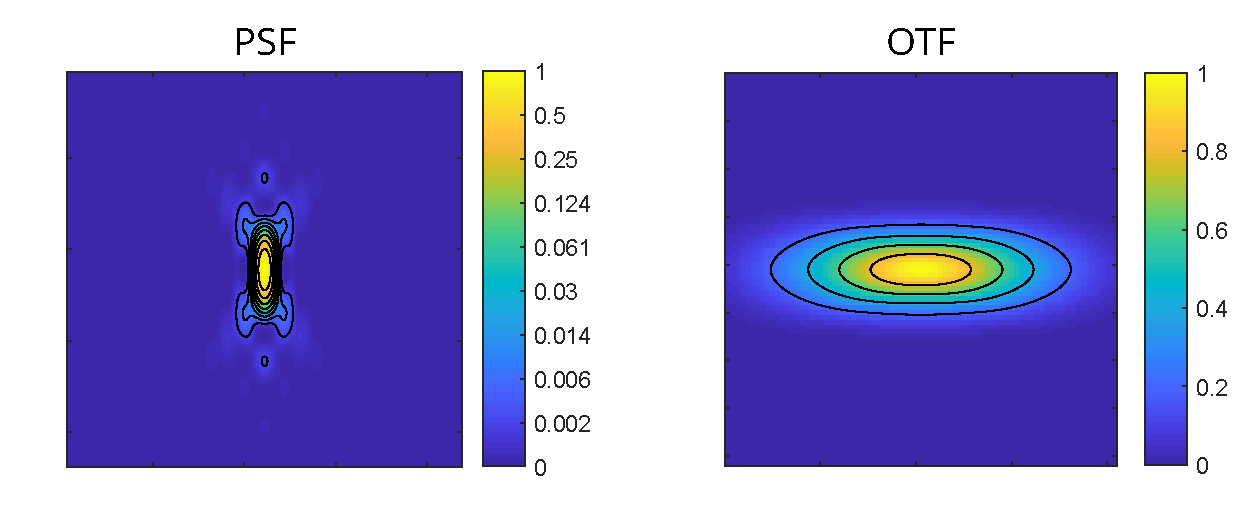
\includegraphics[width=1\textwidth]{psfs/confocal.pdf}
      \bcaption[Axial cross section of the PSF and OTF of a confocal laser scanning microscope]{Simulated PSF and OTF for a laser scanning confocal microscope with a water immersion objective ($n=1.33$). $NA=1.1$, $\lambda = \SI{510}{nm}$}
      \label{fig:psf-confocal}
    \end{figure}


  \subsection{Confocal-theta microscopy}

    % Although confocal microscopy already provides a better resolution in all dimensions, the ratio of the axial and lateral resolution is still very high, due to the single objective illumination and detection. This seriously limits the microscope's 3D imaging capabilities, since in the $z$ direction (i.e. along the imaging axis) the resolution would be significantly worse than in the other directions.
    Although confocal microscopy already has 3D capabilities, its axial resolution is still limited compared to the lateral, since it uses only one objective. An alternative realization of the confocal microscope, the confocal theta microscope \cite{stelzer_fundamental_1994} introduces a second objective to the system, that is used to illuminate the sample (Fig. \ref{fig:conf-theta}). Since this decouples the illumination and detection, using a filter cube is no longer necessary. The second objective is rotated by $\theta$ around the focus, this is where the name of this setup originates from.

    As in the case of standard confocal microscopy, the system PSF is improved by the illumination pattern. Here, however, the axial direction of the detection coincides with the lateral direction of the illumination, which results in a dramatic improvement of axial resolution compared to standard confocal microscopy. Lateral resolution will also be increased, but by a smaller extent, resulting in an almost isotropic PSF, and equal axial and lateral resolutions (Fig. \ref{fig:psf-theta}). 

    Although this is a big improvement to confocal microscopy in terms of resolution, this technique did not reach a widespread adoption as it complicates sample handling, while still suffering from two big drawbacks of confocal microscopy techniques that limits its live imaging capabilities.

    Imaging live specimens for an extended period of time with confocal microscopy although possible \cite{aldaz_live_2010, maitre_asymmetric_2016}, is not ideal. For each voxel imaged, a large portion of the specimen has to be illuminated, which results in a very high dose of radiation on the samples. This can be as much as 30--100 times larger, than the dose used for the actual imaging \cite{reynaud_light_2008}. Illumination with high power of laser for an extended time frame can result in bleaching the fluorophores, which in turn will lower the signal at later times. Furthermore, any absorbed photon has the possibility to disrupt the chemical bonds inside the specimen, which can lead to phototoxic effects. Moreover, the usage of the pinhole although increases resolution, also decreases the detectable signal intensity, thus has a negative impact on image contrast \cite{stelzer_contrast_1998}.

  % \subsection{Mammalian imaging with confocal microscopy}
    


%  ######  ########  #### ##     ## 
% ##    ## ##     ##  ##  ###   ### 
% ##       ##     ##  ##  #### #### 
%  ######  ########   ##  ## ### ## 
%       ## ##         ##  ##     ## 
% ##    ## ##         ##  ##     ## 
%  ######  ##        #### ##     ## 


\section{Light-sheet microscopy}
  \label{sec:light-sheet}
  \begin{figure}[bt]
    \centering
    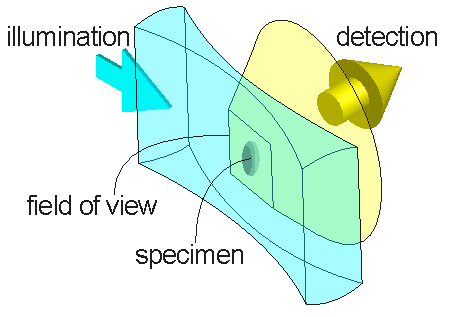
\includegraphics[width=0.6\textwidth]{spim_concept}
    \bcaption[Basic concept of single-plane illumination microscopy]{The sample is illuminated from the side by laser light shaped to a light-sheet (blue). This illuminates the focal plane of the detection lens, that collects light in a wide-field mode (yellow). The image is recorded, and the sample is translated through the light-sheet to acquire an entire 3D stack.}
    \label{fig:spim_concept}
  \end{figure}

  A selective-plane illumination microscope (SPIM) uses a light-sheet to illuminate only a thin section of the sample (Fig.~\ref{fig:spim_concept}). This illumination plane is perpendicular to the imaging axis of the detection objective and coincides with the focal plane. This way, only the section in focus will be illuminated, thus providing much better signal to noise ratio. In case of conventional wide-field fluorescence microscopy, where the whole specimen is illuminated, light scattering from different regions contributes to a significant background noise. With selective-plane illumination, this problem is intrinsically solved, and it also provides a true sectioning capability. This makes SPIM especially suitable for 3D imaging.

  

  The main principle behind single plane illumination microscopy, that is illuminating the sample from the side by a very thin light-sheet, dates back to the early 20\textsuperscript{th} century, when Siedentopf and Zsigmondy first described the ultramicroscope \cite{siedentopf_uber_1902}. This microscope used sunlight as an illumination source, that was guided through a precision slit to generate a thin light-sheet. This allowed Zsigmondy to visualize gold nanoparticles floating in and out of the light-sheet. Since these particles are much smaller than the wavelength of the light, the device was called an ultramicroscope. His studies with colloids, and the development of the ultramicroscope led Zsigmondy to win the Nobel Prize in 1925.

  After Zsigmondy, this method was forgotten until rediscovered in the 1990s, when Voie \etal constructed their Orthogonal-plane Fluorescent Optical Sectioning (OPFOS) microscope \cite{voie_orthogonal-plane_1993}. They used it to image a fixed, optically cleared and fluorescently labelled guinea pig cochlea. In order to acquire a 3D dataset, the sample was illuminated from the side with a light-sheet generated by a cylindrical lens, then rotated around the center axis to obtain multiple views. Although they only reached a lateral resolution around \SI{10}{\micro m} and axial resolution of \SI{26}{\micro m}, this method allowed them to generate a 3D reconstruction of the cochlea \cite{voie_three-dimensional_1995}.

  Later, in 2002, Fuchs et al. developed Thin Light-Sheet Microscopy (TLSM) \cite{fuchs_thin_2002} and used this technique to investigate the microbial life in seawater samples without disturbing their natural environment (by e.g. placing them on a coverslip). Their light-sheet was similar to the one utilized in OPFOS, being \SI{23}{\micro m} thin, and providing a $\SI{1}{mm} \times \SI{1}{mm}$ field of view.

  Despite these early efforts, the method did not gain larger momentum. The real breakthrough in light-sheet imaging happened at EMBL in 2004, where Huisken \etal \cite{huisken_optical_2004} combined the advantages of endogenous fluorescent proteins and the optical sectioning capability of light-sheet illumination to image Medaka fish embryos, and the complete embryonic development of a \textit{Drosopila melanogaster} embryo. They called this Selective-Plane Illumination Microscopy (SPIM), and it quickly became popular to investigate developmental biological questions.

  \label{sec:multiview}
  \begin{figure}[tb]
    \centering
    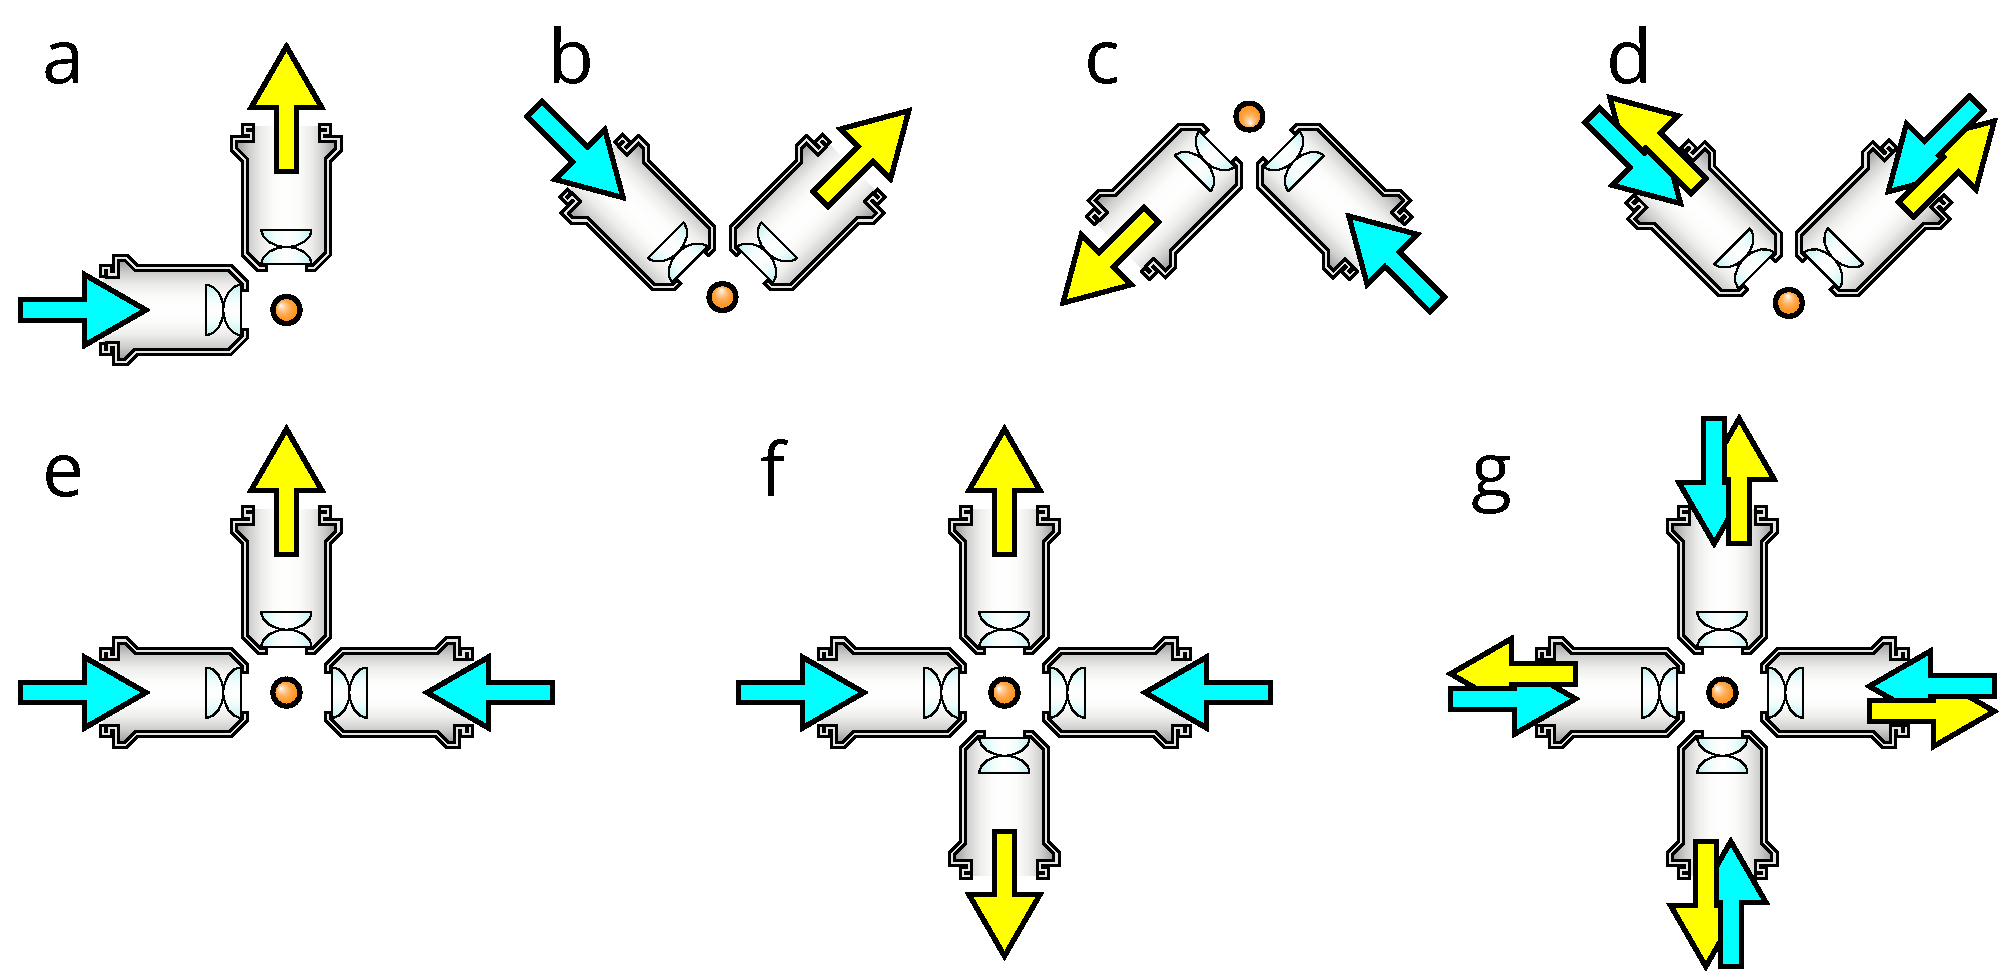
\includegraphics[width=\textwidth]{spim_zoo}
    \bcaption[Different optical arrangements for light-sheet microscopy]{\textbf{(a)} Original SPIM design with a single lens for detection and illumination. \cite{huisken_optical_2004} \textbf{(b)} Upright SPIM to allow for easier sample mounting such as using a petri dish (iSPIM, \cite{capoulade_quantitative_2011, wu_inverted_2011, hoyer_breaking_2016}). \textbf{(c)} Inverted SPIM, where the objectives are below the sample, which is held by a thin foil \cite{strnad_inverted_2016}. \textbf{(d)} Dual-view version of the upright configuration, where both objective can be used for illumination and detection (diSPIM, \cite{wu_spatially_2013}). \textbf{(e)} Multidirectional-SPIM (mSPIM) for even illumination of the sample with two objectives for illumination \cite{huisken_even_2007}. \textbf{(f)} Multi-view SPIM with two illumination and detection objectives for \textit{in toto} imaging of whole embryos (MuVi-SPIM \cite{krzic_multiview_2012}, SimView \cite{tomer_quantitative_2012}, Four-lens SPIM \cite{schmid_high-speed_2013}). \textbf{(g)} A combination of (d) and (f), using four identical objectives, where both can illuminate and detect in a sequential manner, to achieve isotropic resolution without sample rotation (IsoView \cite{chhetri_whole-animal_2015}).}
    \label{fig:spim_zoo}
  \end{figure}
  
  Since then, light-sheet based imaging has gained more and more popularity, as it can be adapted and applied to a wide variety of problems. Although sample mounting can be challenging because of the objective arrangement, this can also be an advantage, since new microscopes can be designed with the sample in mind \cite{huisken_selective_2009, de_medeiros_light-sheet_2016} (Fig. \ref{fig:spim_zoo}). This made it possible to adapt the technique for numerous other specimens, such as zebrafish larvae \cite{keller_reconstruction_2008}, \textit{C. elegans} embryos \cite{wu_inverted_2011}, mouse brain \cite{dodt_ultramicroscopy:_2007}, and even mouse embryos \cite{ichikawa_live_2013, udan_quantitative_2014, strnad_inverted_2016}.

  As many of these specimens require very different conditions and mounting techniques, these microscopes have been adapted to best accommodate them. An upright objective arrangement for example (Fig \ref{fig:spim_zoo}b) allows imaging samples on a coverslip, while its inverted version is well suited for mouse embryos, where a foil is separating them from the immersion medium (Fig. \ref{fig:spim_zoo}c). A modified version of the upright arrangement allows for multi-view imaging using both objectives for illumination and detection in a sequential manner (Fig. \ref{fig:spim_zoo}d) \cite{kumar_dual-view_2014}.

  For larger samples, to achieve a more even illumination, two objectives can be used from opposing directions to generate two light-sheets (Fig. \ref{fig:spim_zoo}e) \cite{huisken_even_2007}. This arrangement can further be complemented by a second detection objective, to achieve parallelized multi-view imaging (Fig. \ref{fig:spim_zoo}f) \cite{krzic_multiview_2012,tomer_quantitative_2012, schmid_high-speed_2013}. For ultimate speed, 4 identical objectives can be used to achieve almost instantaneous views from 4 different directions by using all objectives for illumination and detection (Fig \ref{fig:spim_zoo}g) \cite{chhetri_whole-animal_2015}. 

  Furthermore, because of the wide-field detection scheme it is possible to combine SPIM with many superresolution techniques, such as single molecule localization \cite{cella_zanacchi_live-cell_2011}, STED \cite{friedrich_sted-spim:_2011}, RESOLFT \cite{hoyer_breaking_2016}, or structured illumination \cite{keller_fast_2010,chen_lattice_2014,chang_csilsfm_2017}.


  % things to improve: resolution
  % axial resolution relative to lateral
  % complete view
  % reduce scattering
  
  % implementations to this end:
  % To mSPIM \cite{huisken_even_2007} Fig. \ref{fig:spim_zoo}e, Ultramicroscope from Dodt \textit{et al.} \cite{dodt_ultramicroscopy:_2007}
  
  % upright imaging in petri dish: iSPIM from Wu \textit{et al.} \cite{wu_inverted_2011}, SPIM-FCS Capoulade \textit{et al.} \cite{capoulade_quantitative_2011}, RESOLFT-SPIM Hoyer \textit{et al.} \cite{hoyer_breaking_2016}; Fig. \ref{fig:spim_zoo}b

  % dual-view inverted SPIM, or diSPIM \cite{kumar_dual-view_2014} Fig. \ref{fig:spim_zoo}d

  % inverted SPIM for mouse imaging Strnad \textit{et al.} \cite{strnad_inverted_2016}, Fig. \ref{fig:spim_zoo}c

  % MuVi-SPIM \cite{krzic_multiview_2012}, SimView \cite{tomer_quantitative_2012}, Four-lens SPIM \cite{schmid_high-speed_2013}, Fig. \ref{fig:spim_zoo}f

  % IsoView \cite{chhetri_whole-animal_2015} Fig. \ref{fig:spim_zoo}g
  
  % Bessel beam illumination \cite{fahrbach_line_2010,fahrbach_propagation_2012,fahrbach_light-sheet_2013}, Betzig's Bessel \cite{gao_3d_2014} 2P Bessel Beam from Betzig \cite{planchon_rapid_2011}

  %\begin{itemize}	
  %	\item mSPIM, pivoting light-sheet \cite{huisken_even_2007}
  %	\item omnidirectional microscopy (review) \cite{weber_omnidirectional_2012}
  %	\item SiMView \cite{tomer_quantitative_2012}
  %\end{itemize}


  \subsection{Optics of light-sheet microscopy}

    
    \begin{figure}[htb]
        \centering
        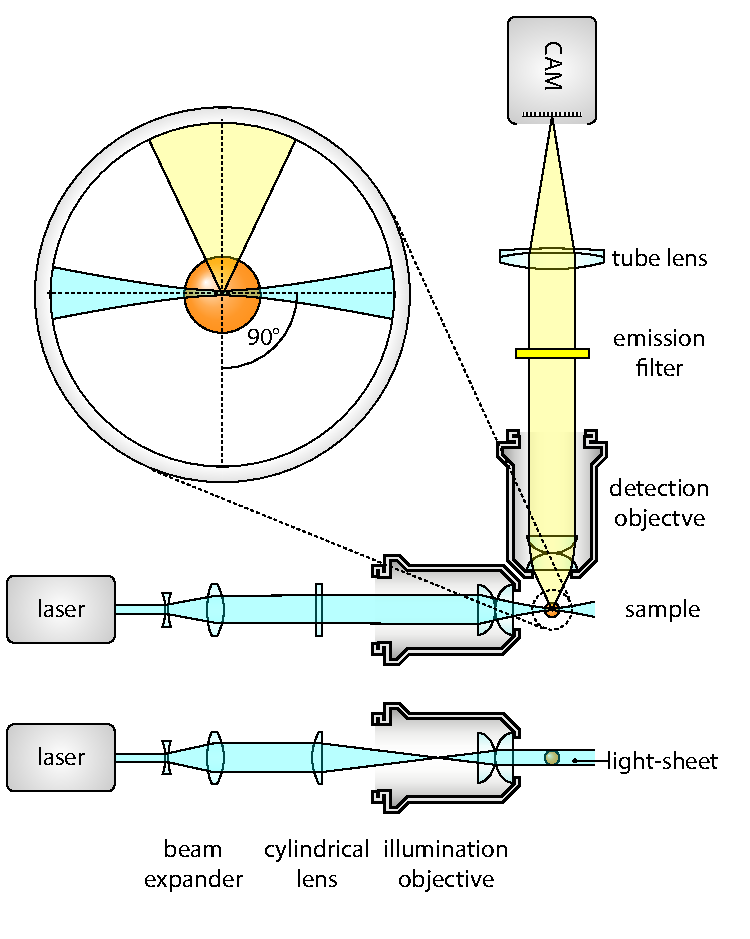
\includegraphics[page=1,width=0.7\textwidth]{spim_cyl}
        \bcaption[Basic optical components of a SPIM]{A dedicated illumination objective is used to generate the light sheet, which is an astigmatic Gaussian beam, focuses along one direction. Astigmatism is introduced by placing a cylindrical lens focusing on the back focal plane of the objective. Detection is preformed at a right angle, with a second, detection objective. Scattered laser light is filtered, and a tube lens forms the image on an area sensor, such as an sCMOS camera.}
        \label{fig:light-sheet}
    \end{figure}

    % \begin{figure}
    %     \centering
    %     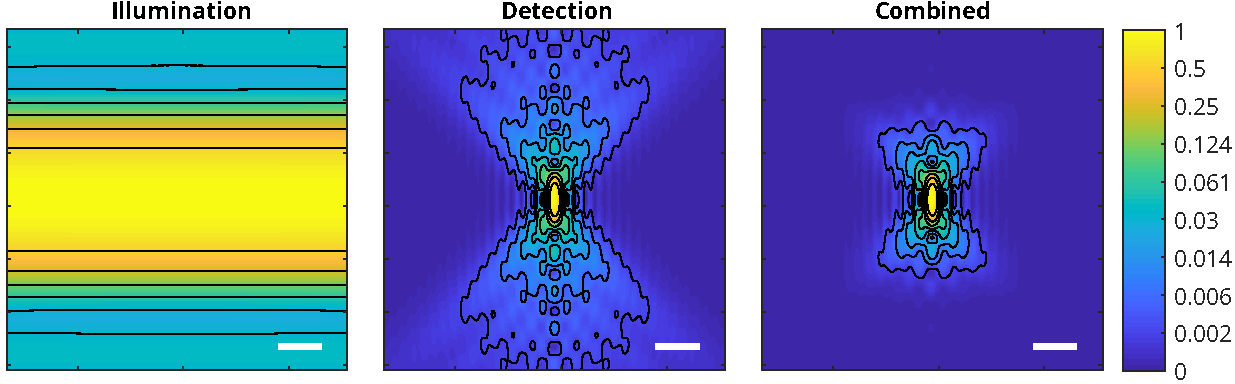
\includegraphics[width=1\textwidth]{psfs/psf_spim.pdf}
    %     \bcaption[Axial cross section of the PSF in a light-sheet microscope]{Simulated PSFs for illumination (left, NA = 0.1, $\lambda = \SI{488}{nm}$) and detection (center, NA=1.1, $\lambda = \SI{510}{nm}$). The system PSF is the multiplication of these PSFs (right).($n=1.33$). Because of the illumination scheme, the light-sheet microscope has a better axial resolution than a conventional wide-field setup.}
    %     \label{fig:psf-spim}
    % \end{figure}


  % \subsection{Detection}
    Since illumination and detection for light-sheet microscopy are decoupled, two independent optical paths are implemented.
    
    The detection unit of a SPIM is basically equivalent to a detection unit of a wide-field microscope, without a dichroic mirror (Fig. \ref{fig:light-sheet}). The most important components are the objective together with the tube lens, filter wheel, and a sensor, typically a CCD or sCMOS camera.

    One of the most important aspects that determines the resolution of the microscope is the detection objective. Since imaging biological specimens usually requires a water-based solution, the objectives also need to be directly submerged in the medium to minimize spherical aberrations. Since the refraction index of water ($n=1.33$) is greater than the refraction index of air, these objectives tend to have a higher NA, which results in higher resolution. The final resolution, however, also depends on the pixel size of the sensor which determines the spatial sampling rate of the image.

    Although image quality and resolution greatly depends on the detection optics, the real strength of light-sheet microscopy, the inherent optical sectioning is due to the specially designed illumination pattern, that confines light to the vicinity of the detection focal plane.

    There are two most commonly used options to generate a light-sheet: either by using a cylindrical lens, to illuminate the whole field of view with a static light-sheet, as in the original SPIM concept \cite{huisken_optical_2004}; or by quickly scanning a thin laser beam through the focal plane, thus resulting in a virtual light-sheet \cite{keller_reconstruction_2008}.


  % \subsection{Illumination}

  \subsection{Static light-sheet illumination}
    For a static light-sheet, the normally circular Gaussian laser beam needs to be shaped in an astigmatic manner, i.e. either expanded or squeezed along one direction, to shape it into a sheet instead of a beam. This effect can be achieved by using a cylindrical lens, which as the name suggests has a curvature in one direction, but is flat in the other, thus focusing a circular beam to a sheet.
    
    However, to achieve light-sheets that are thin enough, one would need to use cylindrical lens with a very short focal length, and these are hardly accessible in well corrected formats. For this reason, it is more common to use a longer focal length cylindrical lens in conjunction with a microscope objective, which is well corrected for chromatic and spherical aberrations \cite{greger_basic_2007}. This way, the light-sheet length, thickness and width can be adjusted for the specific imaging tasks.


    \subsubsection{Light-sheet dimensions}
    \label{sec:dimensions}
    \begin{figure}
      \centering
      \begin{subfigure}[b]{0.29\textwidth}
          \centering
          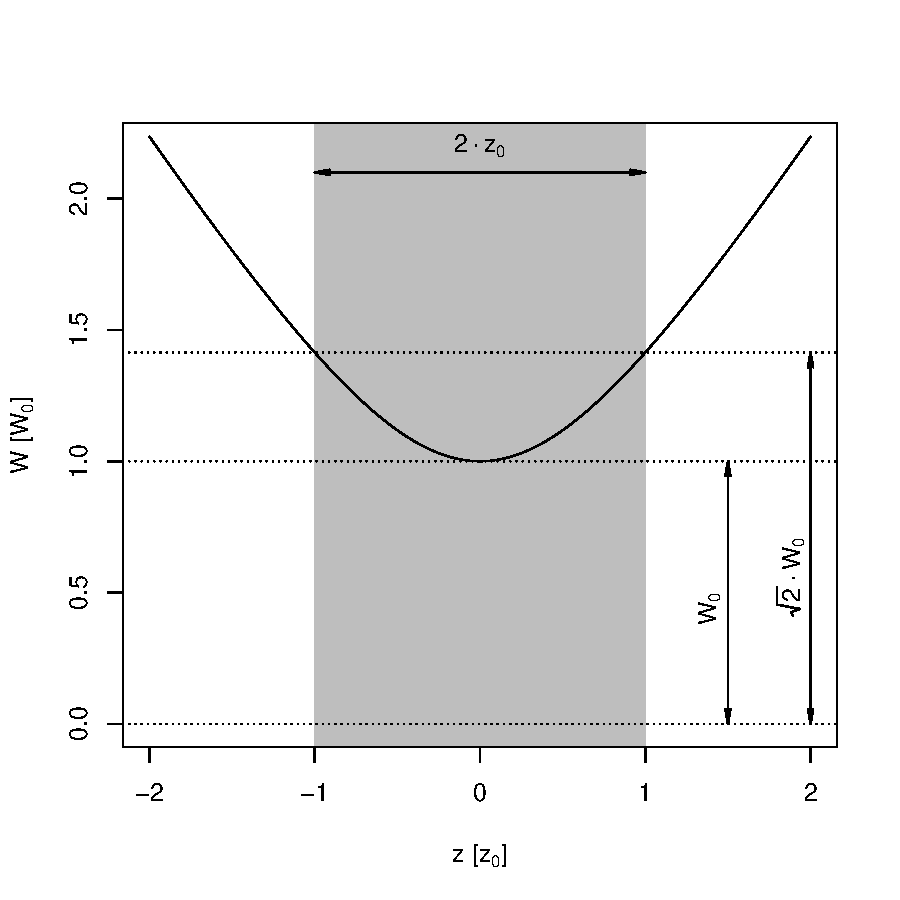
\includegraphics[width=\textwidth]{width}
          \caption{}
          \label{fig:width}
      \end{subfigure}
      \begin{subfigure}[b]{0.29\textwidth}
          \centering
          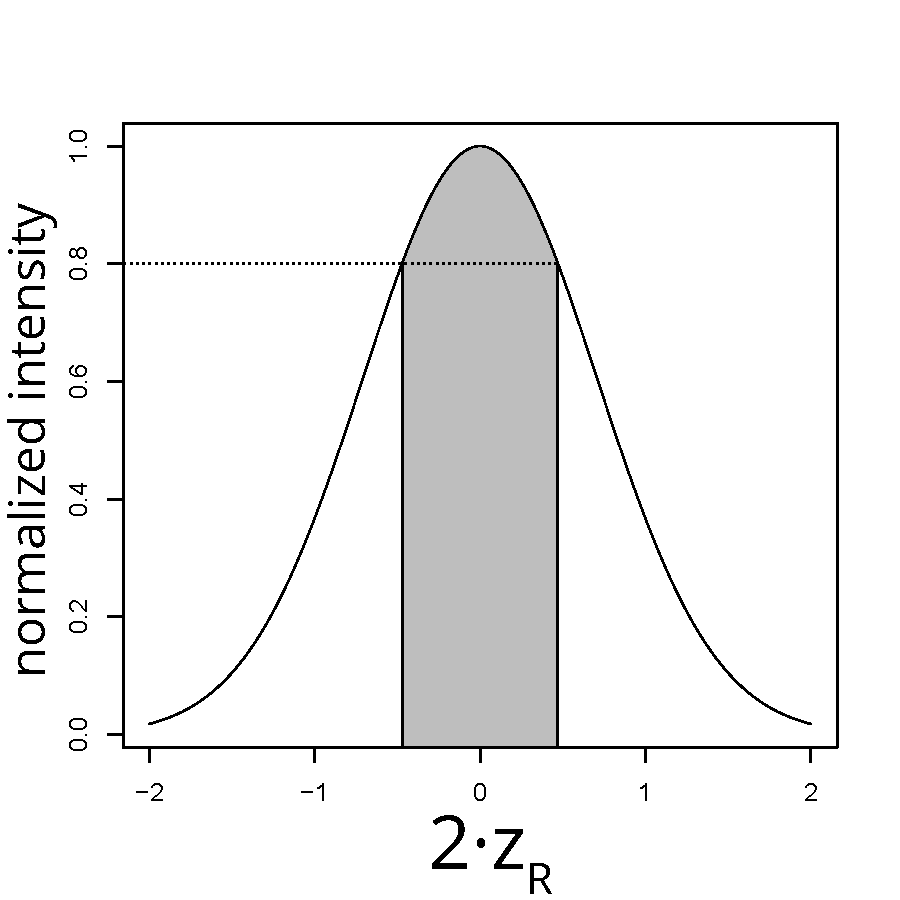
\includegraphics[width=\textwidth]{height}
          \caption{}
          \label{fig:height}
      \end{subfigure}
      \begin{subfigure}[b]{0.39\textwidth}
          \centering
          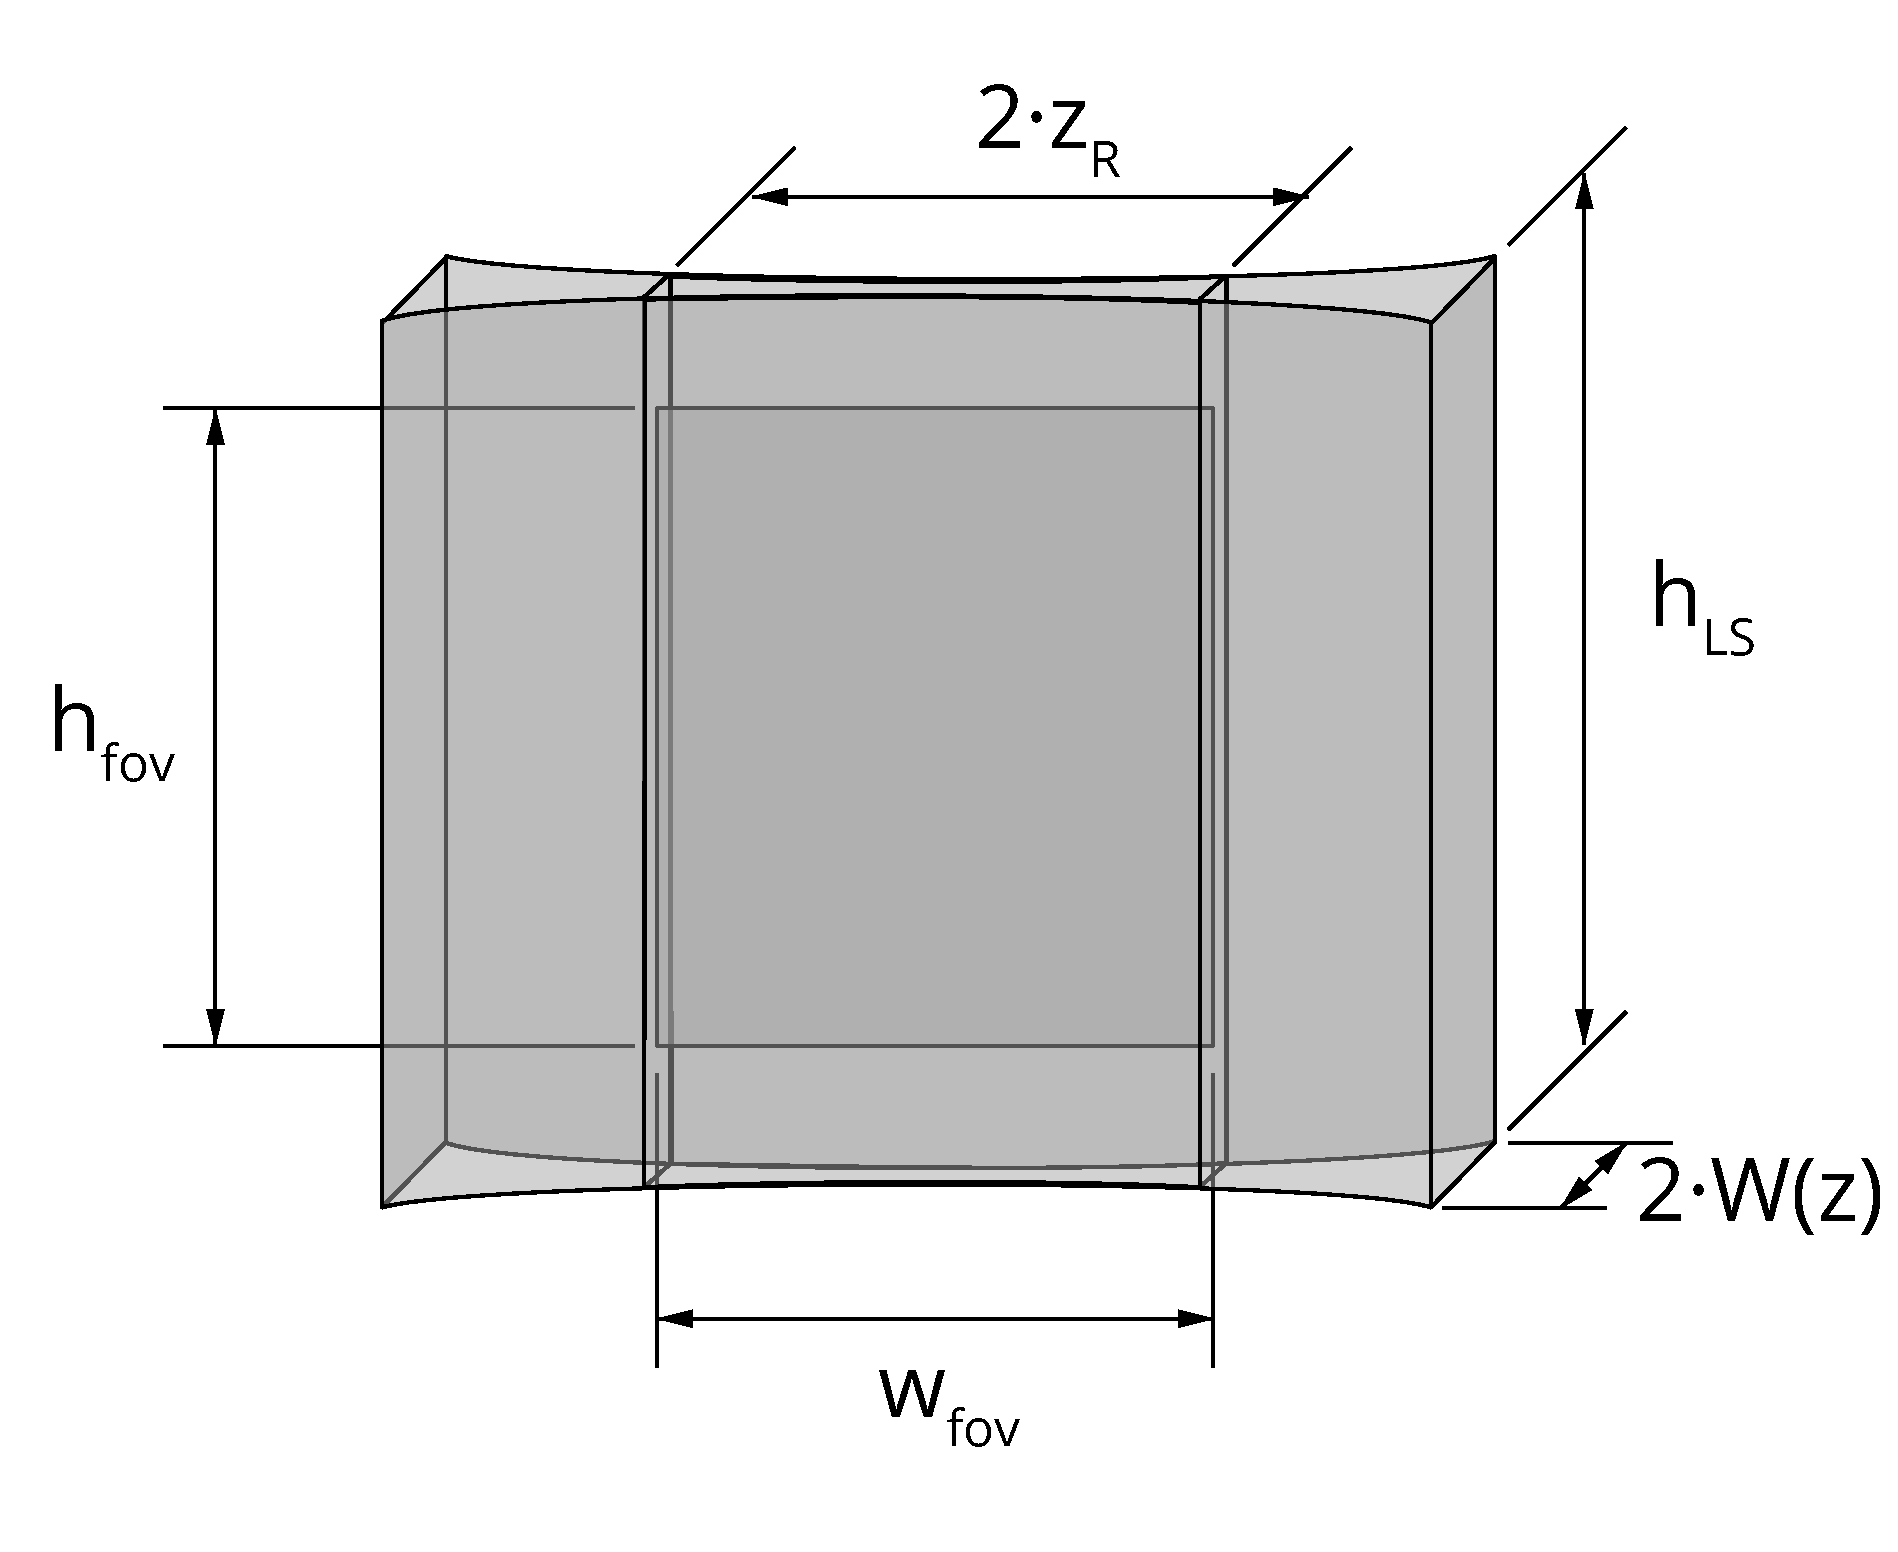
\includegraphics[width=\textwidth]{FOV}
          \caption{}
          \label{fig:fov}
      \end{subfigure}
      \bcaption[Light-sheet dimensions]{ \ref{fig:width} The width and thickness of the field of view depends on the Rayleigh length of the beam ($z_{R,y}$) and the beam waist ($W_0$). \ref{fig:height} Height of the field of view is determined by the Gaussian profile of the astigmatic beam. \ref{fig:fov} shows a light sheet, with the field of view indicated. Since the light-sheet intensity is uneven, the field of view has to be confined to a smaller region. }
      \label{fig:ls_dim}
    \end{figure}

    The shape of the illumination light determines the optical sectioning capability and the field of view of the microscope, so it is important to be able to quantify these measures. The most commonly used illumination source is a laser beam coupled to a single mode fiber, thus its properties can be described by Gaussian beam optics.

    For paraxial waves, i.e. waves with nearly parallel wave front normals, a general wave equation can be approximated with the paraxial Helmholtz equation \cite{saleh_fundamentals_2007}
    \begin{equation}
      \nabla_T^2 U + i 2k \frac{\partial U}{\partial z} = 0
      \label{eq:helmholtz}
    \end{equation}
    where $\nabla_T^2 = \frac{\partial^2}{\partial x^2} + \frac{\partial^2}{\partial y^2}$, $U(\vec{r})$ is the wave function, $k=\frac{2\pi}{\lambda}$ is the wavenumber and $z$ is in the direction of the light propagation.
    
    A simple solution to this differential equation is the Gaussian beam:
    \begin{equation}
      U(r,z) = A_0 \cdot \frac{W_0}{W(z)} \cdot e^{-\frac{r^2}{W^2(z)}}\cdot e^{-i\cdot \phi(r,z)}
    \label{eq:gaussian}
    \end{equation}
    where $A_0$ is the amplitude of the wave, $W_0$ is the radius of the beam waist (the thinnest location on the beam), $r=\sqrt{x^2+y^2}$ is the distance from the center of the beam, $W(z)$ is the radius of the beam $z$ distance from the waist, and $\phi(r,z)$ is the combined phase part of the wave-function (Fig. \ref{fig:width}). Furthermore:

    \begin{equation}
      W(z) = W_0\sqrt{1+\left( \frac{z}{z_R} \right)^2}
    \end{equation}
    where the parameter $z_R$ is called the Rayleigh-range, and is defined the following way:

    \begin{equation}
      z_R = \frac{\pi W_0^2}{\lambda}.
      \label{eq:rayleigh}
    \end{equation}
    

    % The available height of the field of view depends on the uniformity of the illumination. The intensity of the emitted fluorescence is based on the intensity of the excitation light. In case of a Gaussian beam:
    % \begin{equation}
    %   I(r,z) = U(r,z)\cdot U^*(r,z) = |A_0|^2 \cdot \left( \frac{W_0}{W(z)}\right)^2 \cdot e^{-\frac{2r^2}{W^2(z)}},
    % \end{equation}

    Apart from the circular Gaussian beam, the elliptical Gaussian beam is also an eigenfunction of Helmholtz equation (\ref{eq:helmholtz}) which describes the beam shape after a cylindrical lens:
    \begin{equation}
      U(x,y,z) = A_0 \cdot \sqrt{\frac{W_{0,x}}{W_x(z-z_{0,x})}} \sqrt{\frac{W_{0,y}}{W_y(z-z_{0,y})}} \cdot e^{-\frac{x^2}{W_x^2(z-z_{0,x})}} \cdot e^{-\frac{y^2}{W_y^2(z-z_{0,y})}} \cdot e^{-i\cdot \phi(x,y,z)}
    \end{equation}
    This beam still has a Gaussian profile along the $x$ and $y$ axes, but the radii ($W_{0,x}$ and $W_{0,y}$), and the beam waist positions ($z_{0,x}$ and $z_{0,y}$) are uncoupled, which results in an elliptical and astigmatic beam. The beam width can be now described by two independent equations for the two orthogonal directions:
    \begin{align}
      W_x(z) = W_{0,x}\sqrt{1+\left( \frac{z}{z_{R,x}} \right)^2}\mathrm{\quad and \quad } W_y(z) = W_{0,y}\sqrt{1+\left( \frac{z}{z_{R,y}} \right)^2}.
    \end{align}
    Since the beam waist is different along the two axes, the Rayleigh range is also different:
    \begin{align}
      z_{R,x} = \frac{\pi W_{x,0}^2}{\lambda}, \quad
      z_{R,y} = \frac{\pi W_{y,0}^2}{\lambda}.
      \label{eq:rayleighXY}
    \end{align}
    % Intensity of the beam is the following:
    % \begin{equation}
    %   I(x,y,z) = U(x,y,z)\cdot U^*(x,y,z) = |A_0|^2 \cdot \frac{W_{x,0}}{W_x(z)} \cdot \frac{W_{y,0}}{W_y(z)} \cdot e^{-\frac{2x^2}{W_x^2(z)}} \cdot e^{-\frac{2y^2}{W_y^2(z)}}
    % \end{equation}
    
    
    Based on these equations, the light-sheet dimensions and usable field of view (fov) can be specified (Fig. \ref{fig:fov}). The light-sheet thickness will depend on the beam waist, $W_{0,y}$ (if we assume the cylindrical lens is focusing along $y$), and the length of the light-sheet can be defined as twice the Rayleigh range, $2 \cdot z_{R,y}$. As these are coupled (see Eq. \ref{eq:rayleighXY}), having a thin light-sheet for better sectioning also means the length of it will be relatively short. Fortunately, because of the quadratic relation, to increase the field of view by a factor of two, the light-sheet thickness only needs to increase by a factor of $\sqrt{2}$.

    % Since the illumination is uneven, the usable height of the field of view is smaller than the actual illuminated region (Figure \ref{fig:fov}). The width of the field of view $w_{fov}$ is determined by the Rayleigh length, since this is in a direct relation with the beam divergence. To stay in the optimal region, the light-sheet should only be used in the range of 1 Rayleigh length on both sides of the beam waist (Figure \ref{fig:width}). In this range, the ratio between the thickest (at $z=z_0$) and the thinnest (at $z=0$) part of the beam $W(z)$ will be $\sqrt{2}\approx 1.4142$ which is still acceptable.

    Light-sheet height is determined by the intensity profile of the beam along the vertical axis (Fig, \ref{fig:height}). Since this is a Gaussian function (see Eq. \ref{eq:gaussian}), only a small part in the middle can be used for imaging, because towards the sides the intensity dramatically drops. To allow a maximum 20\% drop of intensity at the edges, the light-sheet height is $h_{fov}=2\cdot 0.472\cdot W_{x,0}$.
    

  \subsection{Digitally scanned light-sheet illumination}

    \begin{figure}[bt!]
      \centering
      \includegraphics[page=2,width=0.7\textwidth]{spim_cyl}
      \bcaption[DSLM illumination]{DSLM illuminates a specimen by a circularly-symmetric beam that is scanned over the field of view. This creates a virtual light-sheet, which illuminates a section of a specimen just like the SPIM. Light-sheet in DSLM is uniform over the whole field of view and its height can be dynamically altered by changing the beam scan range.
    }
        \label{fig:dslm}
    \end{figure}

    Although generating a static light-sheet is relatively straightforward, with the simple addition of a cylindrical lens to the light path, it has some drawbacks. As already mentioned in the previous section, the light intensity distribution along the field of view is not constant, as the light-sheet is shaped from a Gaussian beam. Furthermore, along the lateral direction of the light-sheet the illumination NA is extremely low, resulting in effectively collimated light. Because of this, shadowing artifacts can deteriorate the image quality \cite{huisken_even_2007}.

    A more flexible way of creating a light-sheet is by scanning a focused beam in the focal plane to generate a virtual light-sheet (digital scanned light-sheet microscopy, DSLM \cite{keller_reconstruction_2008}). Although this method might require higher peak intensities, it solves both drawbacks of the cylindrical lens illumination. By scanning the beam, the light-sheet height can be freely chosen, and a homogenous illumination will be provided. Focusing the beam in all directions evenly introduces more angles in the lateral direction as well, which shortens the length of the shadows.
    
    The basic optical layout of a DSLM is shown on Fig. \ref{fig:dslm}. A galvanometer controlled mirror is used to alter the beam path that can quickly turn around its axis which will result in an angular sweep of the laser beam. To change the angular movement to translation, a scan lens is used to generate an intermediate scanning plane. This plane is then imaged to the specimen by the tube lens and the illumination objective, resulting in a scanned focused beam at the detection focal plane. The detection unit is identical to the wide-field detection scheme, similarly to the static light-sheet illumination. By scanning the beam at a high frequency, a virtual light-sheet is generated, and the fluorescent signal is captured by a single exposure on the camera, resulting in an evenly illuminated field of view.

  



  



% ##     ##  #######  ##     ##  ######  ######## 
% ###   ### ##     ## ##     ## ##    ## ##       
% #### #### ##     ## ##     ## ##       ##       
% ## ### ## ##     ## ##     ##  ######  ######   
% ##     ## ##     ## ##     ##       ## ##       
% ##     ## ##     ## ##     ## ##    ## ##       
% ##     ##  #######   #######   ######  ######## 
\section{Light-sheet microscopy for mouse imaging}

  Because of its optical sectioning capabilities, combined with the high specificity of fluorescent labels, confocal microscopy had an immense influence on biological research, and has been the go-to technique for decades for many discoveries \cite{shotton_confocal_1989,graf_live_2005,jonkman_any_2015}.
  % Even though it has some drawbacks, important discoveries have been made using this technique, as live imaging is not always necessary.
  % Especially using cell cultures, or fixed specimens, confocal microscopy has been used to investigate X chromosome inactivation \cite{costanzi_histone_1998}, the role of amyloid $\upbeta$-peptide in Alzheimer's disease \cite{bard_peripherally_2000}, the role of Oct4 \cite{nichols_formation_1998} and Sox2 \cite{avilion_multipotent_2003} in the self-renewal of pluripotent stem cells, just to highlight a few.
  Live imaging capabilities of confocal microscopy are, however, limited. This is mostly due to the illumination scheme: to collect information from a single point, almost the whole embryo has to be illuminated. This unwanted illumination can easily lead to bleaching of the fluorophores, and also to phototoxic effects that can prevent further embryonic development. The point scanning nature of image acquisition also implies an inherent constraint to the maximum imaging speed, as it can be only increased at the expense of reducing signal intensity (Fig. \ref{fig:tradeoffs}).

  One improvement to address both of these drawbacks is the use of a spinning disk with a specific pattern (also called Nipkow disk) of holes to generate multiple confocal spots at the same time \cite{graf_live_2005}. If these spots are far enough from each other, confocal rejection of out-of-focus light can still occur. As the disk is spinning, the hole pattern will sweep the entire field of view, eventually covering all points \cite{kino_intermediate_1990}. The image is recorded by an area detector, such as a CCD or EM-CCD, which speeds up image acquisition \cite{nakano_spinning-disk_2002}.

  Although out-of-focus illumination is still an issue, spinning disk confocal microscopy was successfully used to investigate the mechanisms of symmetry breaking in early mouse embryonic development \cite{korotkevich_apical_2017}, and the mechanisms leading to the first cell fate specification that will differentiate extraembryonic tissue form the embryo proper \cite{maitre_pulsatile_2015,dietrich_venus_2015,maitre_asymmetric_2016}. Even though these studies were carried out with live embryos, only a few hours of continuous imaging is possible before the accumulation of phototoxic effects arrests development \cite{nowotschin_chapter_2010}. Compared to this, just the pre-implantation phase of mouse embryonic development spans 3 days, and the full development is 18 days \cite{wolpert_principles_2011}.


  \subsection{Imaging pre-implantation}

    Pre-implantation is the first phase of mouse embryonic development, that starts right after fertilization. The embryo in this phase is still in the oviduct, travelling towards the uterus, where it will implant to the uterine wall. The developmental stage between fertilization and the implantation is called the pre-implantation stage. Here the embryo divides, and already the first cell fate specifications start when forming the trophoectoderm (TE) and the inner cell mass (ICM) at the blastocyst stage. ICM cells will form the embryo proper, while TE cell will contribute to the formation of the extraembryonic tissues.
    
    During this process the embryo is still self-sufficient, which makes it possible to image this stage in an \textit{ex vivo} embryo culture by providing the proper conditions \cite{doherty_culture_2000}. Long term imaging, however, is extremely challenging due to the very high light sensitivity of the specimens. Imaging these embryos in a confocal microscope will lead to incomplete development, even if the imaging frequency is minimized to every \SI{15}{mins} \cite{strnad_inverted_2016}.

    Imaging for just a few hours is already enough to investigate important processes, such as cell fate patterning \cite{dietrich_stochastic_2007}. Other approaches aim to lower the phototoxicity by either using 2-photon illumination which operates at longer wavelengths \cite{denk_two-photon_1990,squirrell_long-term_1999,mcdole_lineage_2011}, or by lowering imaging frequency as a compromise \cite{yamagata_long-term_2009}. These approaches, however either require highly specialized equipment, such as an ultra short pulsed laser, or is compromising on the time resolution.

    Light-sheet microscopy, on the other hand, drastically lowers phototoxic effect by using a much more efficient illumination scheme (see Sec. \ref{sec:light-sheet}), and thus makes a better use of the photon budget. Using this technique, it is possible to image the full pre-implantation development at high spatial and temporal resolution without any negative impact on the developmental process. Such a microscope was developed by Strnad \textit{et al.} at EMBL \cite{strnad_inverted_2016}, who used it to understand when exactly is the first cell fate specification decided in the embryonic cells.

    \begin{figure}[tb]
      \centering
      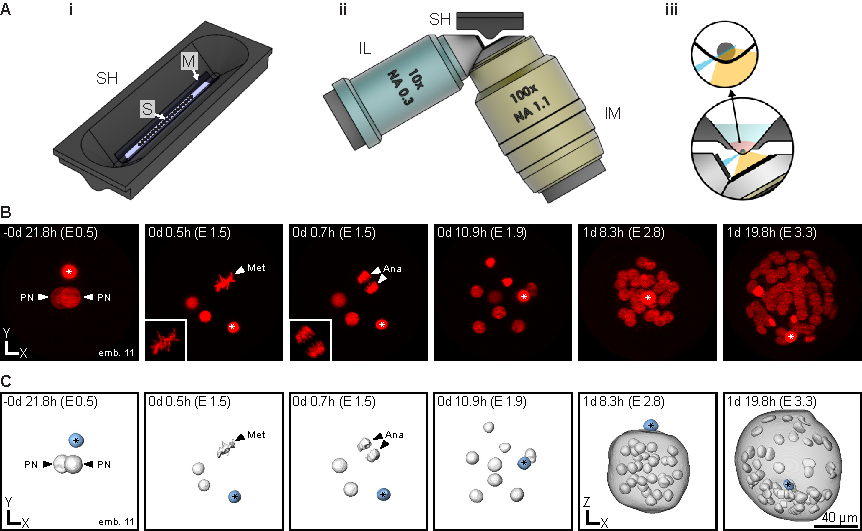
\includegraphics[width=0.8\textwidth]{mammals/Figure2}
      \bcaption[Inverted light-sheet microscope for multiple early mouse embryo imaging.]{(i) A sample holder (SH), containing a transparent FEP membrane (M) allows multiple embryo samples (S) to be placed in line for multisample imaging. (ii) Inverted objective orientation with side view of the sample holder. One possible configuration is to use a 10× 0.3 NA illumination objective (IL) and another 100× 1.1 NA detection objective placed at a right angle to the illumination. (iii) Close up on side view of sample on FEP membrane with both objectives. Since the FEP membrane is transparent on water, it provides no hindrance to the illumination beam in penetrating the sample or for the emitted fluorescence on reaching the detection objective. (B) Still images of one particular timelapse experiment, and (C) corresponding segmented nuclei. The star depicts the polar body. Adapted from Strnad \etal \cite{strnad_inverted_2016}}
      \label{fig:preMouse}
    \end{figure}

    As a mouse embryo culture is not compatible with the standard agarose-based sample mounting techniques, a completely new approach was taken, which resulted in a microscope designed around the sample. The sample holder forming a V-shape was built with a bottom window, and it is lined with a thin FEP (fluorinated ethylene propylene) foil that supports the embryos (Fig. \ref{fig:preMouse}A, i). This arrangement allows the utilization of the standard microdrop embryo culture, while providing proper viewing access for the objectives. As the embryos are relatively small (\SI{100}{\micro m}) and transparent, a single illumination and single detection objective arrangement is enough for high quality imaging. A low resolution (NA=0.3) objective is used to generate the scanned light-sheet, and a high resolution (NA=1.1) objective is detecting the fluorescence at 50\texttimes magnification (Fig \ref{fig:preMouse}A, ii). As the foil is curved, it allows unrestricted access to the embryo, while separating the imaging medium from the immersion liquid (Fig. \ref{fig:preMouse}A, iii). Furthermore, its refractive index is matching the refractive index of water, so optical aberrations are minimized.

    Using this setup, Strnad \textit{et al.} were able to pinpoint the exact timing of the first cell fate decision that leads either to ICM or TE cells. More than 100 embryos expressing nuclear (H2B-mCherry) and membrane (mG) markers were imaged for the entire 3 days of pre-implantation development (Fig. \ref{fig:preMouse}B). The image quality was good enough to segment all nuclei in the embryos (Fig. \ref{fig:preMouse}C), and track them from 1 to 64 cell stage, building the complete lineage tree. Based on the lineage trees, and the final cell fate assignments, it was determined that at the 16 cell stage the final specification is already decided, while earlier than this it is still random.
    

  \subsection{Imaging post-implantation development}
  
    \begin{figure}[tb]
      \centering
      \includegraphics[width=0.8\textwidth]{mammals/Figure3}
      \bcaption[Imaging mouse post-implantation development]{(A) (i, ii) Mounting technique for E5.5 to E6.5 embryos. A tip-truncated \SI{1}{mL} syringe holds an acrylic rod, cut and drilled with holes of different size in order to best fit the mouse embryo by its Reichert's membrane, leaving the embryo free inside the medium. (iii) Maximum intensity projection of a \SI{13}{\micro m} slice at \SI{78}{\micro m} from distal end of an E6.5 mouse embryo. The different tissues corresponding to the rudimentary body plan are annotated. Scale bar: \SI{20}{\micro m}. (B) For stages ranging between E6.5 and E8.5, mounting using a hollow agarose cylinder has also successfully been proposed. Optimal sizes for the corresponding embryonic stage to be imaged can be produced, so that the embryo can grow with least hindrance. (C–F) Steps for mounting the mouse embryo inside the agarose cylinder. The inner volume of the cylinder can be filled with optimal medium, allowing the much larger chamber volume to have less expensive medium. (G–H) Example images of a \SI{9.8}{h} timelapse with the mounting shown in (B) where the expansion of the yolk sac can be observed in direction of the blue arrows. (I) In order to aid multiview light-sheet setups in overcoming the higher scattering properties of embryos at this stage, and to allow faster and easier data recording, electronic confocal slit detection allows better quality images to be taken at shorter acquisition times. Scale bar: \SI{20}{\micro m}. Adapted from Ichikawa \textit{et al.} \cite{ichikawa_live_2013}, Udan \textit{et al.} \cite{udan_quantitative_2014} and de Medeiros and Norlin \textit{et al.} \cite{de_medeiros_confocal_2015}.}
      \label{fig:postMouse}
    \end{figure}

    After the initial 3 days of pre-implantation, the embryo undergoes the implantation process, during which it is inaccessible to microscopical investigations. Although a new method was recently developed that allows \textit{in vitro} culturing of the embryos embedded in a 3D gel \cite{panavaite_3d-geec:_2017}, this has not reached wider adoption yet. Because of this, developmental processes during implantation have only been investigated in fixed embryos.
    
    Following the implantation process, at the post-implantation phase, \textit{ex vivo} embryo culturing becomes possible again \cite{hsu_vitro_1979, huang_effect_2001}, and these embryos can be kept alive for several days in an artificial environment. During this process especially interesting stages are the late blastocyst ($\sim$4.5), gastrulation ($\sim$E6.5), and somite formation ($\sim$E8.5). Before live imaging techniques became available, these stages were mostly investigated using \textit{in situ} visualization techniques to shed light on several developmental processes \cite{nowotschin_cellular_2010}. Many pathways playing important roles have been identified this way, however live imaging is still necessary to validate these results, and ensure continuity in the same specimen \cite{garcia_live_2011}.

    Light-sheet microscopy is a good choice for imaging these stages, just like in the case of pre-implantation embryos. These embryos, however, present new challenges for sample handling and culturing. Owing to their extreme sensitivity, dissection can be difficult, especially for earlier stages (E4.5). Furthermore, since the embryo is also growing during development, gel embedding is not an option, as this might constrain proper development. Thus, special handling and mounting techniques had to be developed in order to allow live 3D imaging of these specimens.

    Ichikawa \textit{et al.} \cite{ichikawa_live_2013} designed a custom mounting apparatus manufactured from acrylic in the shape of a rod that fits in a standard \SI{1}{mL} syringe with its tip truncated (Fig. \ref{fig:postMouse}A, i). In the rod several holes were drilled with different sizes that can accommodate different sized embryos, which are held by an extraembryonic tissue, the Reichert's membrane (Fig. \ref{fig:postMouse}A, ii). Mounting this way doesn't disturb the embryo itself, and it can freely develop in the culturing medium, while it is also stationary for the purpose of imaging. Using this technique, Ichikawa \textit{et al.} were able to image through several stages of development, including interkinetic nuclear migration at stages E5.5--6.5 (Fig. \ref{fig:postMouse}A, iii).

    A second method of sample mounting for light-sheet imaging was developed by Udan~\etal who were able to record a full \SI{24}{h} time-lapse of living embryos focusing on the gastrulation and yolk sac formation processes (Fig. \ref{fig:postMouse}G--I). Their mounting technique comprised of producing a hollow agarose container shaped like a cylinder that could support the embryo from below without constraining its growth (Fig. \ref{fig:postMouse}B--F).

    Another consideration to keep in mind, is the growing size of the embryo. As it gets bigger, illumination is less efficient, and scattering can dominate at larger depths. As mentioned in earlier (Sec. \ref{sec:multiview}) this can be alleviated by multi-view imaging: illuminating and detecting from multiple directions. Electronic confocal slit detection can further improve the signal to noise ratio by rejecting unwanted scattered light, which allows deeper imaging in large specimens, even up to E7.5 (Fig. \ref{fig:postMouse}I) \cite{de_medeiros_confocal_2015}.

  \subsection{Imaging adult mice}
    
    \begin{figure}
      \centering
      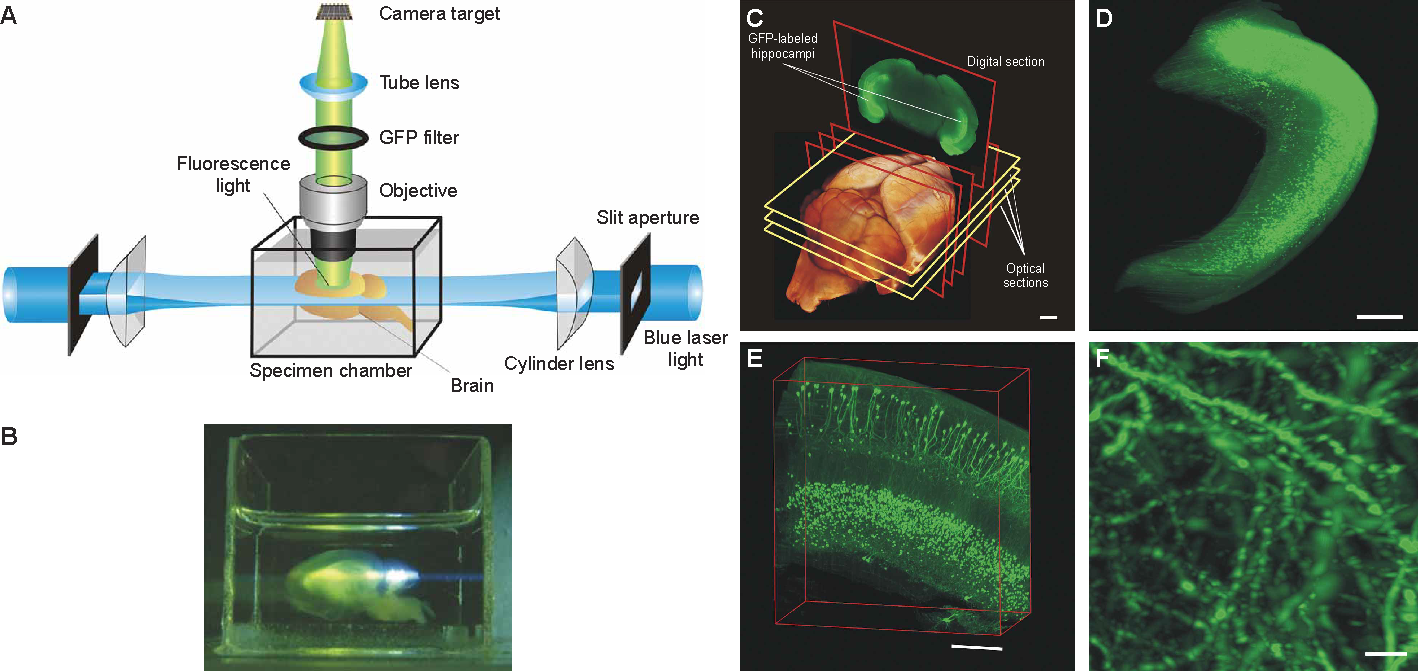
\includegraphics[width=0.8\textwidth]{mammals/Figure4}
      \bcaption[Imaging adult mouse brain with light-sheet microscopy.]{(A) Schematics of the ultramicroscope for brain imaging. The specimen is embedded in clearing medium to ensure necessary imaging depth. Illumination is applied from two sides to achieve even illumination for the whole field of view. Light-sheet is generated by a slit aperture flowed by a cylindrical lens. The specimen is imaged from the top using wide-field detection method. (B) Photograph of the imaging chamber with a mounted cleared specimen and light-sheet illumination. (C) Surface rendering of a whole mouse brain, reconstructed from 550 optical sections. GFP and autofluorescence signal was imaged. Hippocampal pyramidal and granule cell layers are visible in the digital section. Scale bar: \SI{1}{mm}. Objective: Planapochromat 0.5×. (D) Reconstruction of an excised hippocampus from 410 sections. Note that single cell bodies are visible. Scale bar: \SI{500}{\micro m}. Objective: Fluar 2.5×. (E) 3D reconstruction of a smaller region of an excised hippocampus from 132 sections. Scale bar: \SI{200}{\micro m}. Objective: Fluar 5×. (F) 3D reconstruction of CA1 pyramidal cells imaged with a higher resolution objective (LD-Plan Neofluar 20× NA 0.4) in a whole hippocampus (430 sections). Dendritic spines are also visible, even though usually a higher NA objective (>1.2) is required to visualize these. Scale bar: \SI{5}{\micro m}. Adapted from Dodt \textit{et al.} \cite{dodt_ultramicroscopy:_2007}.}
      \label{fig:adultMouse}
    \end{figure}

    Imaging adult mice is especially interesting for answering neurobiological questions. Since development is over at this stage, the use of an environmental chamber is no longer necessary. The biggest challenge for imaging these samples is their size, as they are centimeters in size instead of less than a millimeter in the embryonic stage. Furthermore, the tissues of adult mice are much more opaque which severely limits imaging depth. Light-sheet microscopy can already deal with large specimens, however to achieve (sub)cellular resolution for an entire brain for example, multiple recording have to be stitched together after acquisition \cite{bria_terastitcher_2012}.

    Light scattering and absorption depends on the tissue composition, and also imaging depth. Especially the brain with the high concentration of lipids in the myelinated fibers pose a real challenge for imaging. Live imaging is usually performed with 2-photon microscopy which can penetrate the tissue up to \SI{800}{\micro m} \cite{katona_fast_2012}. Using fixed samples, however, the scattering problem can be eliminated by the use of tissue clearing methods.

    Tissue clearing is a process that removes and/or substitutes scattering and absorbing molecules by a chemical process while keeping the tissue structure intact and preserving fluorescence. The most dominant contributors to these effects are the proteins and lipids. Proteins in the cells locally change the refractive index of the tissue which leads to scattering, while lipids absorb the light. Clearing methods tackle these problems by chemically removing and substituting lipids by certain types of gel, and immersing the whole sample in a medium with higher refractive index to match the optical properties of proteins. Numerous methods have been developed for tissue clearing, such as ScaleA2 \cite{hama_scale:_2011}, 3DISCO \cite{erturk_three-dimensional_2012,erturk_three-dimensional_2012-1}, ClearT2 \cite{kuwajima_cleart:_2013}, SeeDB \cite{ke_seedb:_2013}, CLARITY \cite{chung_clarity_2013,tomer_advanced_2014}, CUBIC \cite{susaki_whole-brain_2014} and iDISCO \cite{renier_idisco:_2014}.

    The first combination of optical clearing and light-sheet microscopy for whole brain imaging was performed by Dodt \etal using a custom ultramicroscope consisting of two opposing illumination arms and a single detection with an objective from above (Fig. \ref{fig:adultMouse}A). The light-sheets were positioned horizontally, and the cleared samples could be placed in a transparent imaging chamber filled with the clearing medium (Fig. \ref{fig:adultMouse}B). Imaging was performed from both top and bottom after rotating the sample \SI{180}{\degree}. By changing the detection lens, it is possible to adapt the system to different samples: low magnification is capable of imaging the whole brain (Fig. \ref{fig:adultMouse}C), while for smaller, dissected parts, such as the hippocampus, higher magnification with higher resolution is more appropriate (Fig. \ref{fig:adultMouse}D). With this configuration individual cell-cell contacts can be recognized (Fig. \ref{fig:adultMouse}E), and even dendritic spines can be visualized (Fig. \ref{fig:adultMouse}F).

    Although light-sheet microscopy is highly suitable for imaging cleared specimens, even entire mice \cite{tainaka_whole-body_2014}, brain imaging in live animals is more challenging due to the standard two-objective setup of a conventional SPIM microscope. Two light-sheet based methods, however offer a solution for this, axial plane optical microscopy (APOM) \cite{li_axial_2014} and swept confocally-aligned planar excitation (SCAPE) \cite{bouchard_swept_2015} both use only a single objective to generate a light-sheet and detect the fluorescence as well. This is done by rotating the detection plane at an intermediate image (APOM), or by rotating both the light-sheet and detection plane simultaneously (SCAPE).



